%for search with vim and okular
\synctex=1


%%=====================================================================================
% Settings
%%=====================================================================================
\newcommand{\mypapersize}{A4}
\newcommand{\mylaterality}{twoside} %% "oneside" or "twoside"
\newcommand{\myparskip}{half}
\newcommand{\myfontsize}{10pt}
\newcommand{\mylinespread}{singlespacing} % e.g.onehalfspacing, doublespacing, singlespacing
\newcommand{\mylanguage}{french} %american

\documentclass[%
  fontsize=\myfontsize,
	paper=\mypapersize,
	parskip=\myparskip,
	DIV=calc,
	headinclude=true,
	footinclude=true,
	open=right,
	appendixprefix=true,	% include appendix?
	bibliography=totoc,		% include an unnumbered unit of bibliography to the table of contents
	BCOR=10mm,        	  % binding correction (depends on how you bind
	\mylaterality,        % alternative: twoside
  \mylanguage
]{scrbook}

%Encoding
\usepackage[utf8]{inputenc}
\usepackage[T1]{fontenc}

\usepackage{float}

% language adaptions
\usepackage[\mylanguage]{babel}

%% general metadata:
\newcommand{\myauthor}{Manon Racine}  %% also used for PDF metadata (hyperref)
\newcommand{\mydocumentsubject}{Projet d'approfondissement}
\newcommand{\mysubject}{AI-enhanced LoRa Based Indoor Localization System}  %% also used for PDF metadata (hyperref)
\newcommand{\myshortsubject}{AI-enhanced LoRa Based Indoor Localization System}  %% also used for PDF metadata (hyperref)
%%\newcommand{\mykeywords}{Pedestrian detection, Deep learning, CNN, BonsEyes, Thermal images}  %% also used for PDF metadata (hyperref)

%% this information is used only for generating the title page:
\newcommand{\myuniversity}{HES-SO Master} %% your university/school
\newcommand{\myfaculty}{HE-Arc} %% your university/school

\newcommand{\mysupervisora}{Dr. Nuria Pazos}
%%\newcommand{\mysupervisorb}{Florian Sauser}

%%\newcommand{\myexpert}{Adrien Birbaumer}
%%=====================================================================================
% Colors
%%=====================================================================================
% includes some colors
\usepackage[table,usenames,dvipsnames]{xcolor}
\usepackage{color, colortbl}


% Define some colors used in the template
\definecolor{grey}{gray}{0.95}
\definecolor{dkgreen}{rgb}{0,0.6,0}

\definecolor{mauve}{rgb}{0.58,0,0.82}
\definecolor{red}{rgb}{1,0,0}
\definecolor{DispositionColor}{RGB}{0, 0, 0}


\definecolor{Red200}{HTML}{EF9A9A}
\definecolor{Red300}{HTML}{E57373}
\definecolor{Red500}{HTML}{ F44336}
\definecolor{Red800}{HTML}{ C62828}

\definecolor{Orange800}{HTML}{ EF6C00}

\definecolor{Teal900}{HTML}{004D40}
\definecolor{Teal800}{HTML}{00695C}
\definecolor{Teal200}{HTML}{80CBC4}


\definecolor{Cyan200}{HTML}{80DEEA}
\definecolor{Cyan800}{HTML}{ 00838F}

\definecolor{Blue900}{HTML}{0D47A1}
\definecolor{Blue800}{HTML}{1565C0}
\definecolor{Blue700}{HTML}{1976D2}
\definecolor{Blue600}{HTML}{1E88E5}
\definecolor{Blue500}{HTML}{2196F3}
\definecolor{Blue400}{HTML}{42A5F5}
\definecolor{Blue300}{HTML}{64B5F6}
\definecolor{Blue200}{HTML}{90CAF9}
\definecolor{Blue100}{HTML}{BBDEFB}

\definecolor{Green900}{HTML}{1B5E20}
\definecolor{Green800}{HTML}{2E7D32}

\definecolor{Grey100}{HTML}{F5F5F5}



%%=====================================================================================
%% includes pictures --> possible to include them in header/footer
%%=====================================================================================
\usepackage[pdftex]{graphicx}


%%=====================================================================================
%% Style
%%=====================================================================================
% override some list packages that they use babel -> see koma script doc
\usepackage{scrhack}

% nicer quotes
\usepackage[%
  autostyle,          % adapts language setting
  strict,             % turns warnings into errors
  english=american    % use american quotes style
]{csquotes}

\usepackage[automark]{scrpage2}							% allows usage of header and footer
\usepackage[perpage, hang]{footmisc} 				% footnote options

\renewcommand{\headfont}{\normalfont\sffamily\color{DispositionColor}}
\renewcommand{\pnumfont}{\normalfont\sffamily\color{DispositionColor}}
\addtokomafont{disposition}{\color{DispositionColor}}
\addtokomafont{caption}{\color{DispositionColor}\footnotesize}
\addtokomafont{captionlabel}{\color{DispositionColor}}

\usepackage{calc} %% used for calculation of header footer etc. ...

%% change page layout
\addtolength{\oddsidemargin}{-.875in}
\addtolength{\evensidemargin}{-.875in}
\addtolength{\textwidth}{1.75in}
\addtolength{\topmargin}{-.875in}
\addtolength{\textheight}{3in}  %1.75

% header and footer
\pagestyle{scrheadings}							% for customization for header and footer
\renewcommand{\chapterpagestyle}{scrheadings}	% include header and footer on chapter pages
\clearscrheadfoot

% http://ctan.uib.no/macros/latex/contrib/koma-script/doc/scrguien.pdf
% page 204
\ihead{\myshortsubject}
\ohead{Public}
\ifoot{\vspace{-0.25cm}\myauthor}
\ofoot{ \vspace{-0.25cm} \thepage}
\automark{chapter}
\setheadsepline[ \textwidth + 5pt ]{1pt} % seperation line for header...
\setfootsepline[ \textwidth + 5pt ]{1pt} % ... and footer
\setkomafont{footsepline}{\color{red}} 	 % change colors of seperation lines
\setkomafont{headsepline}{\color{red}}

%%=====================================================================================
%% Table on Contents
%%=====================================================================================
\setcounter{tocdepth}{2}
\setcounter{secnumdepth}{2} % change la profondeur de numérotation

\usepackage{makecell}

\usepackage{tabulary}
\newcolumntype{K}[1]{>{\centering\arraybackslash}p{#1}}

\usepackage{verbatim}


%%=====================================================================================
%% bibliography with biber/biblatex
%%=====================================================================================
\usepackage[backend=bibtex, %% using "biber" to compile references (instead of "biblatex")
            style=numeric, %% see biblatex documentation
            style=alphabetic, %% see biblatex documentation
            backref=true, %% create backlings from references to citations
            natbib=true, %% offering natbib-compatible commands
            hyperref=true,
            sorting=none, %% using hyperref-package references
]{biblatex}

%\addbibresource{../bib/bibliography.bib}
\addbibresource{bib/bibliography.bib}
%\addbibresource{bib/bibliography_VAL.bib}

%%=====================================================================================
%% SIUNITSX -- simplified usage of SI-units
%%=====================================================================================
%\usepackage[
%            group-digits=false,
%            exponent-product = \cdot, % use \cdot instead * for exponent product
%            binary-units=true,
%            load-configurations=binary,
%            load-configurations=abbreviations,
%]{siunitx}

% Easy typesetting hex and bin and oct
\usepackage[autolanguage, nosepfour]{numprint}
\usepackage{nbaseprt}

%%=====================================================================================
%% ifthen and todonotes puts to-do-notes in the printed document if you want
%%=====================================================================================
%% used to disable todonotes package
\usepackage{ifthen}
\newboolean{myaddlistoftodos}
\newboolean{showconfidential}

\reversemarginpar %To display the todo in the right margin
\setlength{\marginparwidth}{2cm} %To correct the bad placement

\usepackage[english]{todonotes}

%%=====================================================================================
%% Tables, figures, enums, etc...
%%=====================================================================================
%% nice rule's for tables try \toprule \midrule \bottomrule
\usepackage{booktabs}

%% set width of table and more
\usepackage{tabularx}										% creates tables

%% rotate tables and figures
\usepackage{rotating}

%% define caption style
\addtokomafont{caption}{\small} 	% small captions
\usepackage[font=small, width=0.9\textwidth, format=plain, labelfont=bf]{caption}

%%
\usepackage{subfigure}
\usepackage{placeins}

%% customize item look
\usepackage{enumitem}

%%=====================================================================================
%% some utility stuff
%%=====================================================================================
% improved typographical settings
\usepackage[%
    protrusion=true, %
    factor=900       %
]{microtype}

%% switch of extra space after punctuation
\frenchspacing

%% switches to Palatino with small caps and old style figures
\usepackage[%
            sc,%
            osf,%
]{mathpazo}

%% kills space between items
\setlist{noitemsep}

%doc% For additional special characters available by \verb#\ding{}#
\usepackage{pifont}  %% Sonderzeichen fuer Titelseite \ding{}

%doc% This package is required for intelligent spacing after commands
\usepackage{xspace}

%doc% This package offers strikethrough command \verb+\sout{foobar}+.
\usepackage[normalem]{ulem}

%% prevent club & widow penalty
\clubpenalty10000
\widowpenalty10000
\displaywidowpenalty10000

%% Titlepage
\usepackage{tcolorbox}


%%=====================================================================================
%% lslistening: used to include source code
%%=====================================================================================
\usepackage{listings}				% include source code

\lstset{% 							% options for representation of source code
  backgroundcolor=\color{grey},   % choose the background color; you must add \usepackage{color} or \usepackage{xcolor}
  basicstyle=\footnotesize,        % the size of the fonts that are used for the code
  breakatwhitespace=false,         % sets if automatic breaks should only happen at whitespace
  breaklines=true,                 % sets automatic line breaking
  captionpos=b,                    % ses the caption-position to bottom
  commentstyle=\color{dkgreen}, % comment style
  deletekeywords={...},            % if you want to delete keywords from the given language
  escapeinside={\%*}{*)},          % if you want to add LaTeX within your code
  frame=lines,                     % adds a frame around the code
  keepspaces=true,                 % keeps spaces in text, useful for keeping indentation of code (possibly needs columns=flexible)
  keywordstyle=\color{blue},       % keyword style
  language=C,                      % the language of the code
  morekeywords={*,...},            % if you want to add more keywords to the set
  numbers=left,                    % where to put the line-numbers; possible values are (none, left, right)
  numbersep=8pt,                   % how far the line-numbers are from the code
  numberstyle=\tiny\color{gray},   % the style that is used for the line-numbers
  rulecolor=\color{black},         % if not set, the frame-color may be changed on line-breaks within not-black text (e.g. comments (green here))
  showspaces=false,                % show spaces everywhere adding particular underscores; it overrides 'showstringspaces'
  showstringspaces=false,          % underline spaces within strings only
  showtabs=false,                  % show tabs within strings adding particular underscores
  stepnumber=1,                    % the step between two line-numbers. If it's 1, each line will be numbered
  stringstyle=\color{blue},        % string literal style
  tabsize=2,                       % sets default tabsize to 2 spaces
  title=\lstname,                  % show the filename of files included with \lstinputlisting; also try caption instead of title
}

%theme for C
\lstdefinestyle{C}{
	language=c, showspaces=false,
	keywordstyle=		\color{blue}\scriptsize,
	commentstyle=	  \color{dkgreen}\scriptsize\sffamily,
	stringstyle=		\color{mauve}\scriptsize,
	title=\lstname,
	escapeinside={//(*}{*)},
	morekeywords={},
	numbers = left, numberstyle=\tiny\color{black}
}

\usepackage{setspace} 
\usepackage{blindtext}
\usepackage{graphicx}
\usepackage[export]{adjustbox}

\usepackage[top=2.5cm, bottom=3cm, left=2.5cm, right=2cm]{geometry}

%%=====================================================================================
%% pdfcompresslevel from 0 to 10; std is fine
%%=====================================================================================
\pdfcompresslevel=9

%%=====================================================================================
%% Hyperref should always be the last package added --
%%=====================================================================================
\usepackage{hyperref}								% should be the last package to be inlcuded!

%\usepackage[%							% enables typesettings for hyperlinks
%pdftitle={\mysubject},%
%pdfauthor = {\myauthor},%
%pdfsubject = {\mysubject},%
%colorlinks={false},
%pdfcreator={pdfTex},%
%pdfkeywords={\mykeywords},%
%pdftex = true,%
%backref,%
%pagebackref=false, % creates backward references too
%bookmarks=True, %
%bookmarksopen=false, % when starting with AcrobatReader, the Bookmarkcolumn is opened
%pdfpagemode=UseOutlines,% None, UseOutlines, UseThumbs, FullScreen
%plainpages=false % correct, if pdflatex complains: ``destination with same identifier already exists''
%]{hyperref}								% should be the last package to be inlcuded!

%---------------------------------------------------------------------------------------------------
% include figures
%---------------------------------------------------------------------------------------------------
\newcommand{\myfigsrc}[5]{
\begin{figure}[htp]
	\begin{center}
		\includegraphics[width=#2\textwidth]{figures/#1}
		\captionsource{#3}{#4}
		\label{#5} %% NOTE: always label *after* caption!
	\end{center}
\end{figure}
}

\newcommand{\myfig}[4]{
\begin{figure}[htp]
	\begin{center}
		\includegraphics[width=#2\textwidth]{figures/#1}
		\caption[#3]{#3}
		\label{#4} %% NOTE: always label *after* caption!
	\end{center}
\end{figure}
}

\newcommand{\mypdfsrc}[6]{
\begin{figure}[htp]
	\begin{center}
		\includegraphics[page=#6, width=#2\textwidth, frame]{figures/#1}
		\captionsource{#3}{#4}
		\label{#5} %% NOTE: always label *after* caption!
	\end{center}
\end{figure}
}


\newcommand*{\captionsource}[2]{%
\caption[{#1}]{%
	#1%
	\\\hspace{\linewidth}%
	\textbf{Source:} #2%
}%
}




%% ========================================================================
%%  TODO: Enable/Disable
%% ========================================================================
\setboolean{myaddlistoftodos}{false}  %% "true" or "false"
%% If set to "true": the current list of open todos is added after the
%% table of contents. If \mytodonotesoptions is set to "disable", no
%% list of todos is added, independent of this setting here.


%----------------------------------------------------------------------------------------
%	\begin{document}
%----------------------------------------------------------------------------------------
\begin{document}

\frontmatter

\begin{titlepage}
	
	% MSE + HES-SO Images
	\vspace{-1cm}
	\begin{minipage}{0.49\textwidth}
		\begin{flushleft} \large
			
\includegraphics[width=0.8\textwidth]{figures/titlepage_fig/mse.pdf}
		\end{flushleft}
	\end{minipage}
	\begin{minipage}{0.5\textwidth}
		\begin{flushright} \large
			
\includegraphics[width=0.6\textwidth]{figures/titlepage_fig/hesso2.pdf}
		\end{flushright}
	\end{minipage}
	
	% HES-SO Master postal address
	\begin{flushleft}
		\footnotesize 		
		Master of Science HES-SO in Engineering\\
		Av. de Provence 6\\CH-1007 Lausanne
	\end{flushleft}
	
	% Vertical space under HES-SO Master postal address
	\vspace{1.7cm}
	
	\begin{flushright}
		{\huge Master of Science HES-SO in Engineering}
		
		\vspace{0.5cm}
		{\Large Orientation : Technologies de l’information et de la communication (TIC)}
		
		\vspace{1.7cm}

		\begin{spacing}{2.0}
			{\Huge \mysubject}
		\end{spacing}

		\vspace{1cm}
		\begin{spacing}{2.0}	
			Fait par\\
			{\huge \myauthor}
		\end{spacing}
	
		
		\vspace{1cm}
		\begin{spacing}{1.5}
			Sous la direction de\\
			{\Large \mysupervisora }\\ 
			%{\Large \mysupervisorb }
		\end{spacing}
	
		{\Large \myfaculty}

%		\begin{spacing}{1.5}
%			Expert externe\\
%			{\Large \myexpert }
%		\end{spacing}
		
		\vspace{1cm}%% Date
		{\large St-Imier, HE-Arc, \today}
	\end{flushright}
	% Bottom of the page
\end{titlepage}
\cleardoublepage
%\chapter*{Soumission du projet}
Accepté par la HES-SO//Master (Suisse, Lausanne) sur proposition de

\vspace{0.5cm}
Dr. Nuria Paszos conseillère de travail de Master

\vspace{2cm}
St-Imier, le 18.09.2018

\vspace{1.5cm}
\begin{minipage}[t]{0.5\textwidth}
	\raggedright
	Dr. Nuria Pazos\\
	Conseillère
\end{minipage}%
\begin{minipage}[t]{0.45\textwidth}
%	\raggedleft
	Prof. Didier Rizzotti\\
	Responsable de la filière MRU-TIC
\end{minipage}




\cleardoublepage

%----------------------------------------------------------------------------------------
%	Abstract
%----------------------------------------------------------------------------------------
\chapter{Résumé}
Ce document présente une analyse de sécurité axée sur le bus CAN d'un véhicule autonome conçu par la société Navya.

Les premiers chapitres décrivent une analyse de l'état de l'art des moyens de communication utilisés dans les véhicules, qu'ils soient autonomes ou à conduite manuelle, puis se focalisent ensuite sur les communications employant le bus CAN, en expliquant les problèmes de sécurité qui peuvent être rencontrés en se basant sur les concepts généraux du chiffrement des télécommunications. 

Cette analyse explore ensuite l'architecture d'un véhicule autonome et la problématique en cas d'accès physique au bus CAN qui n'est pas protégé nativement contre les intrusions et attaques diverses.

Ensuite, des mesures physiques sur le bus CAN contrôlant la direction du véhicule démontrent effectivement la transmission en clair des informations, sans vérification de l'intégrité.

Pour terminer, différentes solutions applicables sont présentées, ainsi qu'une proposition de surcouche pour un bus CAN permettant de garantir l'intégrité et l'authentification des données transférées.
disposition de la documentation nécessaire.

{\let\clearpage\relax\par \chapter{Abstract}}
Dafuq is that report ?
\chapter{Remerciements}
Dans un premier temps, je tiens à remercier chaleureusement Mme Nuria Pazos qui a suivi mon travail minutieusement et qui y a investi de son temps. Elle a été d'un soutien précieux avec toujours un mot d'encouragement positif. 
\\[0.2in]

Sans la collaboration de mon ancien collègue Michael Mueller, la reprise de sa thèse de Master aurait été bien plus compliquée.Il a été d'un grand soutien dans les premiers pas de ce projet. 
\\[0.2in]

Ensuite, j'aimerais dire un tout grand merci à mes collègues qui m'ont aidé de près ou de loin avec leurs conseils et leur partage d'idées. Un merci particulier à Arnaud Gay Des Combes et Olivier Gloriod qui m'ont apporté un soutien considérable dans le langage Python. 
\\[0.2in]

Un merci également à notre très cher concierge Pierre pour avoir laissé mon installation en place ainsi que les scotches de repère durant de longues semaines malgré le dérangements occasionés.
\\[0.2in]

Pour terminer avec une note d'humour, je tiens à remercier mon chat qui m'a servi de bouillotte durant mes longues soirées de rédaction. 



%\chapter{Remerciements}
Merci Jackie
%\chapter*{Déclaration}

\noindent Je, soussigné, \myauthor, déclare sur l’honneur que le travail rendu, intitulé \enquote{\mysubject} est le fruit d’un travail personnel. Je certifie ne pas avoir eu recours au plagiat ou à toutes autres formes de fraudes. Toutes les sources d’information utilisées et les citations d’auteur ont été clairement mentionnées.


\vspace{2cm}

%% definition of the block tat contains date and signature
\newcommand{\mysignatureblock}[3]{%
	%% Sorry, this is a "bit" of a hack. Maybe someone knows a more elegant method?
	\begin{tabular}{llp{2em}l} 
		#1 & \hspace{4cm}        & & \hspace{4cm} \\\cline{2-2}\cline{4-4}
		&                     & & \\[-3mm]
		& {\footnotesize #2}  & & {\footnotesize #3}
	\end{tabular}
}

\mysignatureblock{St-Imier,}{Date}{Signature}



%----------------------------------------------------------------------------------------
%	List of Contents/Figures/Tables
%----------------------------------------------------------------------------------------
\tableofcontents
\listoffigures

\ifthenelse{\boolean{myaddlistoftodos}}{
  \newpage\todototoc \listoftodos          %% handy if you are using todonotes with \todo{}
}{}

%----------------------------------------------------------------------------------------
%	Body
%----------------------------------------------------------------------------------------
\mainmatter

% Chapter file here
%
%\chapter{Rapport intérmédiaire : 17.09.2018 au 12.10.2018}

Ce premier résumé a pour but de poser le projet et d'étudier l'état de l'art. Depuis les lectures concernant ce qu'il existe en machin learning pour le positionnement indoor, il est nécessaire de faire un résumé afin de choisir le meilleur algorithme afin d'améliorer le positionnement indoor à l'aide de la technologie LoRa et le mode ranging.

\section{Cahier des charges}
\subsection{Introduction}
Les systèmes de localisation basés sur GPS souffrent de la détérioration de la précision et sont presque indisponibles dans les environnements intérieurs. Pour les environnements intérieurs, de nombreuses technologies de systèmes de positionnement ont été conçues sur la base de la vision, de la détection infrarouge ou ultrasonore, des champs magnétiques de la terre, des accéléromètres / gyromètres, des balises BLE ou de la communication WiFi. Chacune de ces technologies existantes a des coûts, une précision et un compromis maximum en matière de couverture, mais un service de localisation intérieur générique reste difficile à obtenir.

\subsection{But du projet}
S'appuyant sur les capacités étendues des nouveaux circuits intégrés LoRa, ce projet développera et déploiera un système de localisation capable d'améliorer la précision de la position atteinte par les systèmes de localisation basés sur LoRa existants reposant sur des mécanismes TDOA ou de télémétrie. À cette fin, une exploration et une comparaison des différentes techniques "machine learning/deep learning" pour le positionnement basé sur le "fingerprinting" seront effectuées.


\subsection{Objectifs et tâches à réaliser}
\begin{enumerate}
	\item Etudier le cahier des charges
	\item Etudier l’état de l’art des techniques à utiliser dans le cadre du projet, en particulier les systèmes de localisation indoor basés sur des techniques d’apprentissage, et réunir une documentation (env. 20% effort)
	\item Etablir un planning pour l’ensemble du projet.
	\item Définir un plan des tests à effectuer.
	\item Définir les procédures de test
	\item Définir le setup pour la collecte de données de localisation
	\item Prise en main de l’environnement de développement pour les phases de training et du test de la technique d’apprentissage retenue (e.g., PyTorch).
	\item Implémentation de la solution ML retenue.
	\item Tester le système selon le protocole préétabli.
	\item Faire des propositions pour améliorer les performances de l’algorithme et, si possible, les implémenter.
	\item Rédiger le rapport et documenter l’ensemble du projet.
\end{enumerate}


\section{Résumé du document 00}
Ce document décrit la localisation sans utiliser le GPS et en utilisant LoRa. Il a surtout été utile d'utiliser ce document pour la gestion des "outliers"
\\
\\
Le problème principal avec le GPS c'est la consommation et la durée de vie c'est pourquoi un système basé sur LoRa a été étudié. La portée en milieu rural est d'environ 15km alors qu'il est de 5km dans un milieu urbain cela grâce à la bonne sensibilité du récepteur (-130dBm). Une chose intéressant est la bande passante qui est plus large que d'autres technologies qui permet de distinguer différents chemins du même signal. Sagemcom ont obtenus des bons résultats au niveau de la précision qui est de environ 4 mètres. 
\\
\\
Ce qui est intéressant c'est dans cette publication c'est la manière de traiter les "outliers - valeurs aberrante, c'est-à-dire les points qui ne sont pas cohérent lors d'une mesure. Selon Barnet et Lewis [11], un "outliers" est définit comme étant une observation qui semble incompatible avec le reste d'un ensemble de données.
Garder un "outliers" dans une set de données peut amener à de mauvais résultat il est donc important de les détecter correctement. Il existe différentes méthodes pour déterminer ces "outliers" :

\begin{enumerate}
	\item Grubbs' test : Détecte un "outliers" en supposant une distribution normale.
	\item Tietjen-Moore test : C'est une généralisation de Grubbs' test pour détecter de multiple outliers. Il a cependant un inconvénient, il est nécessaire de connaitre le nombre exact d'ouliers.
	\item Generalized Extreme Studentized Deviate (ESD): C'est également une généralisation du test Grubbs' mais il n'est pas nécessaire de connaitre à l'avance le nombre d'ouliers. Ce test nécessite uniquement une limite supérieure pour le nombre suspect d'outliers.[01]
\end{enumerate}

[11] V. Barnett; T. Lewis, Outliers in Statistical Data, 3rd ed. Wiley Series in Probability and Mathematical Statistics, 1994.

[01] lien concernant les ESD : https://www.itl.nist.gov/div898/handbook/eda/section3/eda35h3.htm

\section{Résumé du document 01}
Cette publication parle d'une analyse comparative entre différents algorithmes de "machine learning" pour du positionnement indoor. L'étude est basée sur un positionnement "fingerprint" ce qui permet de cartographier un endroit à l'aide du de la force du signal récéptionné (RSS - Received Signal Strength).
Dans cet article, les algorithmes de "machine learning" sélectionnés sont comparés en termes de précision de positionnement et de temps de calcul. la base de donnée UJIIndoorLoc a été utilisé pour les différentes expérimentation. Les résultats expérimentaux révèlent que l’algorithme k-Nearest Neighbor (k-NN) est le plus approprié lors du positionnement.

\subsection{Introduction}
Au cours des expériences, la base de données UJIIndoorLoc, qui est préparée pour les systèmes de positionnement à l'intérieur [8], est utilisée. La classification est effectuée en premier lieu en utilisant le jeu de données d'origine en considérant les valeurs RSS de 520 points d'accès sans fil (WAP) et les nouveaux attributs définis en tant que «cellule» qui composent les attributs BuildingID, Floor, SpaceID et RelativePos. Ensuite, une nouvelle méthode est proposée: «Séparation déductive pour le positionnement intérieur (DESIP - Deductive Separation for Indoor Positioning)». Dans cette méthode, tout d'abord, seules les informations de bâtiment et les valeurs RSS mesurées à partir de 520 WAP sont utilisées pour la tâche de classification.
\\
\\
Durant les expériences, des algorithmes déterministes tels que le plus proche voisin (NN - nearest neighbor), le SMO, l'arbre de décision (J48) et des algorithmes probabilistes tels que Naïve Bayes et Bayes Net sont utilisés. L’algorithme le plus approprié pour la solution du problème de positionnement intérieur est déterminé en comparant la précision et le temps de calcul de chaque approche.
\\
\\
La base de données entière est séparée de telle sorte que 19.937 enregistrements soient réservés à la formation et 1.111 enregistrements soient réservés aux tests. Il y a 529 caractéristiques et ces caractéristiques sont les coordonnées où sont prises les empreintes digitales WiFi, telles que bâtiment, étage, espace (bureau, laboratoire, etc.), position relative (dans une pièce ou dans un couloir), etc. Le jeu de données de formation UJIIndoorLoc comprenant les valeurs RSS de 520 WAP et un nouvel attribut «cellule» qui compose les attributs floor, buildingID, spaceID et relative position de l'ensemble de données d'origine est utilisé pour la tâche de classification. Les étapes des expériences utilisant ce jeu de données sont illustrées à la figure \ref{fig:newAttribute}.

\begin{figure}[H]
	\begin{center}
		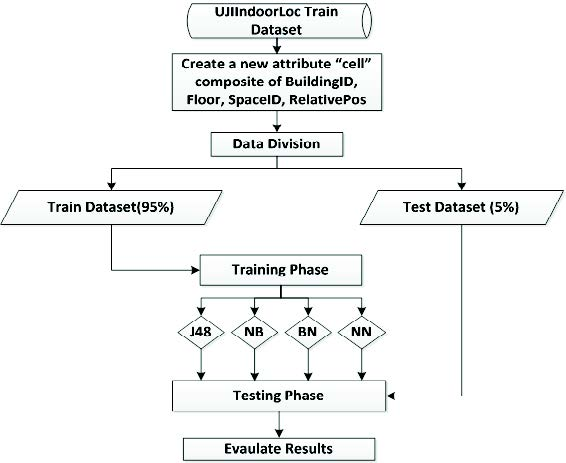
\includegraphics[scale=1]{figures/newattribute.jpg}
		\caption{The new attribute “cell” construction phase}
		\label{fig:newAttribute} %% NOTE: always label *after* caption!
	\end{center}
\end{figure}


\subsection{Algorithmes}
Dans la section suivante, les algorithmes de classification utilisés dans cette étude sont brièvement décrits.

\subsubsection{Decision Tree}
L'arbre de décisions et une méthode très connue en "machine learning". Il possède des noeuds de décisions (non-terminal), des branches, et des noeuds feuilles (terminal) qui représentent les caractéristiques, condition et les classes. A chaque noeud de décision on sait quelle branches suivre et lorsque l'algorithme atteint un noeud final, le label contenu dans ce même noeud est retourné comme étant la classe. 
L’ID3 de Quinlan et son successeur, C4.5, sont les plus populaires parmi les algorithmes d’arbre de décision [19].

(19) J. R. Quinlan, “ C4. 5: programs for machine learning”, Elsevier, 2014.

\subsubsection{Naïve Bayes}
Le classificateur Naïve Bayes [22] basé sur le théorème de Bayes est un algorithme d'apprentissage supervisé [23]. Il est robuste aux données bruyantes, facile à construire, affiche une grande précision et rapidité lorsqu'il est appliqué à de grandes bases de données et exécute des modèles de classification plus complexes. Par conséquent, il est largement utilisé dans les tâches de classification. Il calcule la probabilité de chaque attribut dans les données en supposant qu'elles sont également importantes et indépendantes les unes des autres. Cette hypothèse est appelée indépendance conditionnelle de classe [24, 25].
\\
\\
(22) G. H. John, and P. Langley, “Estimating Continuous Distributions in Bayesian Classifiers”, 11th Conference on Uncertainty in Artificial Intelligence, pp., 338-345, 1995.

(23) C. Anuradha, and S. Dhall, "Software Defect Prediction Using Supervised Learning Algorithm and Unsupervised Learning Algorithm", 2013.

(24) W. Yotsawat, and A. Srivihok, "Inbound tourists segmentation with combined algorithms using K-Means and Decision Tree”, 10th International Joint Conference on Computer Science and Software Engineering (JCSSE), pp.189-194, 2013.

(25) S. Ureerat, and P. Singsri, "The classifier model for prediction quail gender after birth based on external factors of quail egg", IEEE 11th International Joint Conference on Computer Science and Software Engineering (JCSSE), 2014.

\subsubsection{Bayesian Network}

L'algorithme de réseau bayésien est largement utilisé pour la classification et est basé sur le théorème de Bayes où la probabilité conditionnelle sur chaque nœud est calculée et forme un réseau bayésien. Il s'appelle également réseau de croyance ou réseau occasionnel. Réseau bayésien a deux parties nommées qualitatives et quantitatives, qui sont la structure topologique du réseau bayésien et le tableau de probabilité conditionnelle (CPT), respectivement [26].

Le réseau bayésien est un graphe acyclique dirigé où chaque nœud représente un attribut des données et un ensemble de distributions de probabilité. Ces distributions donnent les probabilités pour la valeur de chaque nœud étant donné que les parents de nœud.

(26) D. Yang, and L. Jin-lin, "Research on personal credit evaluation model based on bayesian network and association rules", 2007 International Conference on Wireless Communications, Networking and Mobile Computing, 2007.

\subsubsection{K-Nearest Neighbor}
Le classificateur K-Nearest Neighbor (K-NN) [27] est également connu sous le nom de classificateur basé sur la distance qui classe les instances en fonction de leur similarité. C'est l'un des algorithmes les plus populaires de l'apprentissage automatique. C'est un type d'apprentissage paresseux dans lequel la fonction n'est approchée que localement et tout calcul est retardé jusqu'à la classification. Le tuple inconnu dans K-NN est assigné à la classe la plus commune parmi ses K-plus proches voisins. Lorsque K = 1, le tuple inconnu se voit attribuer la classe du tuple d'apprentissage le plus proche dans l'espace des motifs [28].

(27) D. W. Aha, D. Kibler , and M. K. Albert, “ Instance-based learning algorithms”, Machine Learning, vol. 6, pp., 37-66, 1991.

(28) C. Shah, and A. G. Jivani, "Comparison of data mining classification algorithms for breast cancer prediction", 2013 Fourth International Conference on Computing, Communications and Networking Technologies (ICCCNT), pp.1-4, 2013.

\subsubsection{SMO}
L'algorithme d'optimisation séquentielle minimale (SMO - Sequential minimal optimization) [29] est représenté par John C. Platt pour la formation du classificateur de vecteurs de support à l'aide des noyaux polynomiaux ou RBF. C'est l'un des algorithmes les plus courants pour la classification des grandes marges par SVM. Il remplace globalement toutes les valeurs manquantes et transforme les attributs nominaux en attributs binaires. La SVM est une technique de classification basée sur la technologie des réseaux neuronaux utilisant la théorie de l'apprentissage statistique [30]. Il recherche un hyperplan optimal linéaire afin de maximiser la marge de séparation entre la classe positive et la classe négative. En pratique, la plupart des données ne sont pas linéairement séparables; ainsi, pour rendre la séparation possible, la transformation est effectuée à l'aide d'une fonction du noyau. L'entrée est transformée en un espace caractéristique de dimension supérieure à l'aide d'une cartographie non linéaire [30]. Une décision sur la fonction du Kernel est nécessaire pour implémenter SVM. Le Kernel définit la classe de fonction [31].

[29] J. Platt, “Fast Training of Support Vector Machines using Sequential Minimal Optimization”, Advances in Kernel Methods - Support Vector Learning, 1998.

[30] P. Niken, and H. Ohwada, "Applicability of machine-learning techniques in predicting customer defection", IEEE 2014 International Symposium on Technology Management and Emerging Technologies (ISTMET), 2014.

[31] S. M. Obaidullah, K. Roy, and N. Das, "Comparison of different classifiers for script identification from handwritten document", 2013 IEEE International Conference on Signal Processing, Computing and Control (ISPCC), pp.1-6, 2013.

\subsubsection{AdaBoost}
AdaBoost (Adaptive Boosting) [32] est un algorithme d'apprentissage d'ensemble. Généralement, il peut être utilisé avec des algorithmes de Machine learning faibles pour améliorer leurs performances. Il est simple à mettre en œuvre, rapide et moins susceptible d'avoir un overfitting. Il améliore les algorithmes de classification instables tels que J48, DecisionStump, etc. L'idée derrière cet algorithme est d'obtenir un classificateur très précis en combinant de nombreux classificateurs faibles. Il fonctionne en exécutant de manière répétée un algorithme d'apprentissage faible donné sur diverses distributions sur les données d'apprentissage, puis en combinant les classificateurs produits par l'apprenant faible en un classificateur composite unique [33]. Les classificateurs de l'ensemble sont ajoutés un par un, de sorte que chaque classificateur suivant est entrainé sur des données difficiles pour les membres précédents de l'ensemble. Les poids sont définis sur les instances du jeu de données, en suivant une règle selon laquelle les instances difficiles à classer prennent plus de poids. Cette règle conduit les classificateurs ultérieurs à se concentrer sur eux [34].

[32] Y. Freund, and R. E. Schapire, “Experiments with a new boosting algorithm”, 3th International Conference on Machine Learning, San Francisco, pp. 148-156, 1996.

[33] R. Shams, and R. E. Mercer, "Classifying Spam Emails Using Text and Readability Features", 2013 IEEE 13th International Conference on Data Mining (ICDM, pp. 657-666, 2013.

[34] S. O. Sharif, L. I. Kuncheva, and S. P. Mansoor, "Classifying encryption algorithms using pattern recognition techniques", 2010 IEEE International Conference on Information Theory and Information Security (ICITIS), , pp. 1168-1172, 2010.

\subsubsection{Bagging}
le Bagging [35] crée des sacs de données de la même taille que le jeu de données d'origine en appliquant une sélection aléatoire à différents sous-ensembles des données d'apprentissage avec de nombreux exemples qui apparaissent plusieurs fois. Ce processus est appelé réplication bootstrap des données d'entrainement. L'idée derrière cette technique est de construire différents classificateurs en utilisant ces sous-ensembles. Chaque sous-ensemble est utilisé pour entrainer un classificateur individuel. Cette approche d'ensemble utilise le nombre de classificateurs a priori [35].

[35] L. Breiman, “Bagging predictors”, Machine Learning. vol. 24, no. 2, pp.123-140, 1996.

\subsection{Conclusions}
Dans cet article les algorithme suivant ont été comparé : NN, SMO, J48, Naïve Bayes and BayesNet.

Lorsque tout le dataset est pris en compte, c'est l'algorithme J48 qui est le meilleur :

\begin{figure}[H]
	\begin{center}
		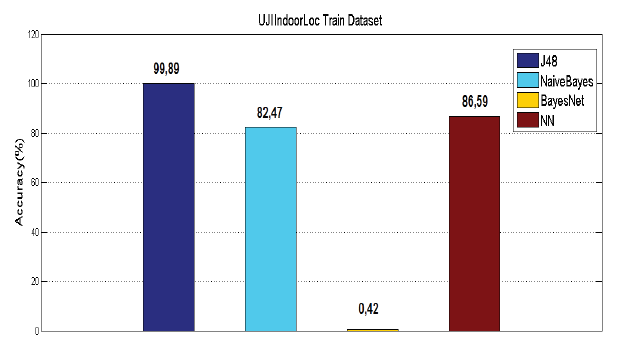
\includegraphics[scale=1]{figures/wholeDataset.png}
		\caption{Accuracy results of classification using whole dataset}
		\label{fig:wohledataset} %% NOTE: always label *after* caption!
	\end{center}
\end{figure}

Ensuite, en accordance à l'approche DESIP (Deductive Separation for Indoor Positioning), la classification est effectuée en 3 phases (building,floor and region). Le resultat des algorithme pour cette classification donne BayesNet comme étant le meilleur.

\begin{figure}[H]
	\begin{center}
		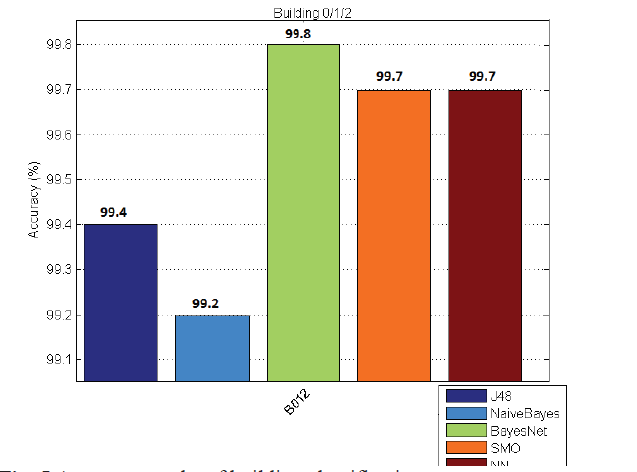
\includegraphics[scale=1]{figures/bluildingClassification.png}
		\caption{Accuracy results of building classification}
		\label{fig:builClass} %% NOTE: always label *after* caption!
	\end{center}
\end{figure}

Suite à cela la classification a été faite en fonction des étages (floors). Dans ce cas le meilleur algorithme est NN. 

\begin{figure}[H]
	\begin{center}
		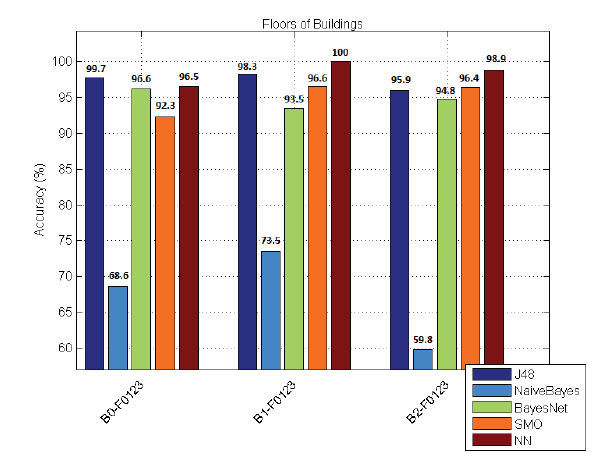
\includegraphics[scale=1]{figures/floorClassification.png}
		\caption{Accuracy results of floor classification}
		\label{fig:floorClass} %% NOTE: always label *after* caption!
	\end{center}
\end{figure}

Et pour la dernière étape, la classification a été faite en fonction de la région et là encore c'est l'algorithme NN qui est le meilleur.

\begin{figure}[H]
	\begin{center}
		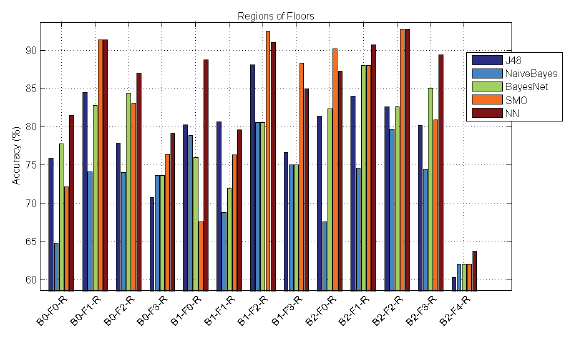
\includegraphics[scale=1]{figures/regionClassification.png}
		\caption{Accuracy results of region classification}
		\label{fig:regionClass} %% NOTE: always label *after* caption!
	\end{center}
\end{figure}

Si les deux tableaux ci-dessous sont analysés, l'algorithme NN est le meilleurs pour tous les dataset niveau temps d'execution. En ce qui concerne la précision, Bayes Net est meilleur pour la classification "building" par contre NN est meilleur dans tous les autres cas.

\begin{figure}[H]
	\begin{center}
		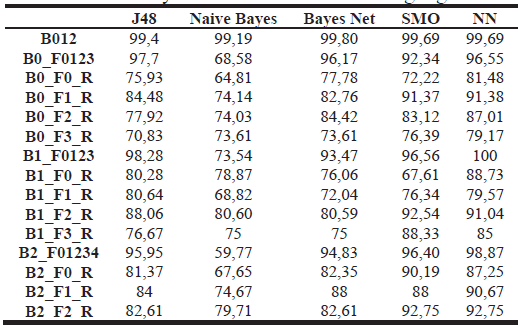
\includegraphics[scale=1]{figures/accuracy.png}
		\caption{Accuracy results of machine learning algorithms}
		\label{fig:accuracy} %% NOTE: always label *after* caption!
	\end{center}
\end{figure}

\begin{figure}[H]
	\begin{center}
		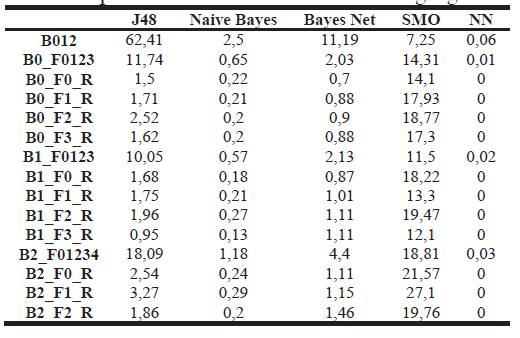
\includegraphics[scale=1]{figures/time.png}
		\caption{Elapsed time results of machine learning algorithms}
		\label{fig:time} %% NOTE: always label *after* caption!
	\end{center}
\end{figure}

De cette publication en découle que NN est supérieur à toutes les autres méthodes pour estimer la position. En outre, J48 offre des performances quasiment identiques lorsqu'il est utilisé avec des algorithmes itératifs, à savoir AdaBoost et Bagging.

\section{Résumé du document 02}
Cette publication traite de la diminution de erreur du mode ranging concernant la localisation UWB (ultra wide band). Plusieurs techniques existent pour diminuer l'erreur de positionnement en détectant ce qui est en ligne de vue (LOS) ou non (NLOS). Ici, il est exploité une autre technique qui va directement diminuer cet erreur que ça soit en LOS ou NLOS. Ils appliquent deux classes de régresseurs non paramétriques pour avoir une estimation de l'erreur de mesure. Afin de valider leurs résultats ils ont fait un vaste campagne de mesures intérieures. Cette technique montre une amélioration de performances significatives dans divers scénarios par rapport aux approches conventionnelles. 

Ils se sont appuyé sur des outils de Machine Learning, et proposent deux techniques de régression non paramétriques pour estimer l’erreur de mesure, en se basant uniquement sur la forme d’onde reçue et la distance estimée.


\begin{enumerate}
	\item La première technique utilise une régression de machine à vecteurs de support (SVM - support vector machine) pour trouver un hyperplan qui se rapproche de l'erreur de mesure en fonction des données d'apprentissage. 
	\item La seconde technique utilise un processus gaussien (GP) pour déterminer la distribution a posteriori de l'erreur de mesure, en fonction des données d'apprentissage. 
\end{enumerate}

L'erreur de mesure estimée, associée à une mesure de certitude, peut être transmise à un algorithme de localisation. Leurs techniques de régression présentent l'avantage supplémentaire de pouvoir être appliquées même lorsque les données d'apprentissage ne sont pas étiquetées avec des informations LOS ou NLOS.

\subsection{Ranging Errors}
Lors de mesure il existe beaucoup de paramètres qui peuvent créer une erreur. Avec un seul model il est difficile de capturer tout les types de perturbations. Dans cette publication, ils se basent sur 1024 mesures (512 LOS et 512 NLOS).

\begin{figure}[H]
	\begin{center}
		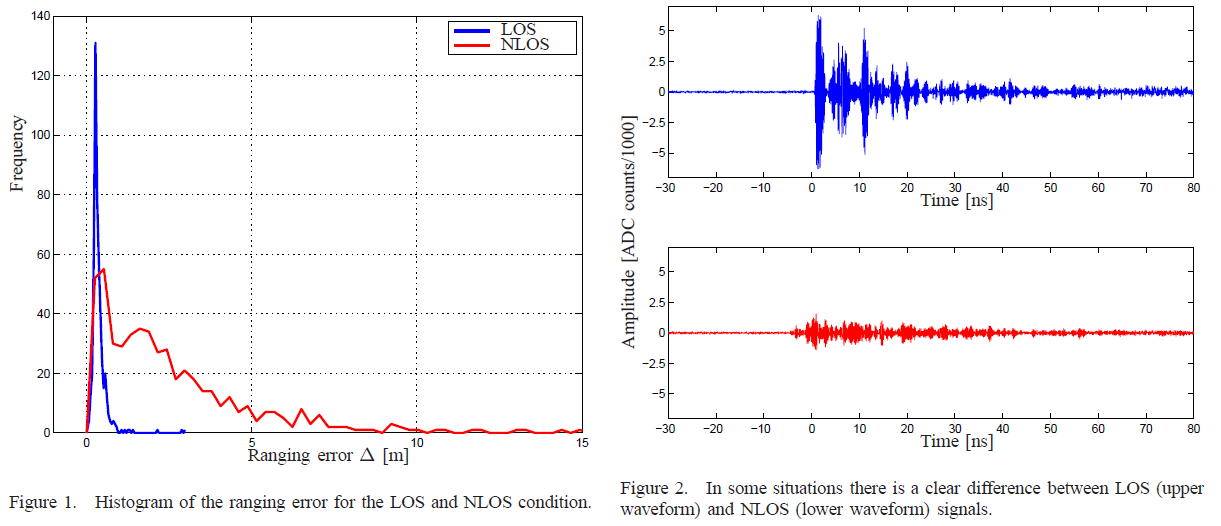
\includegraphics[scale=1]{figures/LosNlos.png}
		\caption{Ranging error - LOS and NLOS}
		\label{fig:LosNlos} %% NOTE: always label *after* caption!
	\end{center}
\end{figure}

Suite, aux différentes mesures et différentes observations dans leur article, ils décident de ne pas labéliser les signaux en LOS et NLOS.

\subsection{Algrorithme}
\subsubsection{Regression with Support Vector Machines}
\subsubsection{Regression with Gaussian Processes}

\subsection{Conclusion}
Les approches classiques pour faire face au défi de la localisation dans des environnements encombrés impliquent généralement d'abord la détection de la condition NLOS, puis la prise de mesures appropriées pour prendre en compte la condition NLOS. Toutefois, la grande variété de matériaux et d’environnements d’exploitation variés peuvent impacter les performances de la mesure de ranging, ce qui indique que la distinction entre LOS et NLOS n’est pas toujours significative. Sur la base de cette observation, ils ont adopté pour une approche différente dans cet article. Leur approche utilise des techniques de Machine Learning non paramétriques (SVM et GP) pour estimer l’erreur de "ranging" directement à partir de la forme d’onde reçue, sans aucune connaissance a priori ou a posteriori de la condition NLOS. 

Sur la base d'une vaste campagne de mesures en intérieur avec des radios UWB conformes à la FCC, ils ont évalué les performances de localisation en termes de probabilité de panne pour différentes stratégies de localisation. Leurs résultats ont révélé que: 

\begin{enumerate}
	\item La minimisation de l1-norme est plus robuste pour faire face aux valeurs aberrantes (outliers) que la minimisation de l2-norme, pour une localisation sans atténuation.
	\item les contraintes peuvent générer des gains significatifs, en particulier lorsque les exigences de localisation ne sont pas trop strictes.
	\item les techniques de régression SVM ou GP offrent des gains de performance supplémentaires pour tous les scénarios considérés.
	\item Les techniques de régression SVM ou GP, combinées à la connaissance des contraintes relatives à l'erreur de "ranging", offrent les meilleures performances pour les scénarios considérés.
\end{enumerate}

\section{Résumé du document 03}
\subsection{Pro/con}
%\chapter{Rapport intérmédiaire : 15.10.2018 au 26.10.2018}

\section{Compostion du dataset UJIIndoorLoc}

Le dataset utilisé pour de nombreux cas de positionnement indoor afin de valider et tester les algortihmes est composé des attributs suivants: 

Attribute 001 (WAP001): Intensity value for WAP001. Negative integer values from -104 to 0 and +100. Positive value 100 used if WAP001 was not detected.

....

Attribute 520 (WAP520): Intensity value for WAP520. Negative integer values from -104 to 0 and +100. Positive Vvalue 100 used if WAP520 was not detected.

Attribute 521 (Longitude): Longitude. Negative real values from -7695.9387549299299000 to -7299.786516730871000

Attribute 522 (Latitude): Latitude. Positive real values from 4864745.7450159714 to 4865017.3646842018.

Attribute 523 (Floor): Altitude in floors inside the building. Integer values from 0 to 4.

Attribute 524 (BuildingID): ID to identify the building. Measures were taken in three different buildings. Categorical integer values from 0 to 2.

Attribute 525 (SpaceID): Internal ID number to identify the Space (office, corridor, classroom) where the capture was taken. Categorical integer values.

Attribute 526 (RelativePosition): Relative position with respect to the Space (1 - Inside, 2 - Outside in Front of the door). Categorical integer values.

Attribute 527 (UserID): User identifier (see below). Categorical integer values.

Attribute 528 (PhoneID): Android device identifier (see below). Categorical integer values.

Attribute 529 (Timestamp): UNIX Time when the capture was taken. Integer value. 

Ces données sont surtout utilisée avec des algorithmes de classification qui ne sera probalement pas notre cas mais cela donne une bonne idée des paramètres qui peuvent être utiles.

Il serait bien de tester un des algorithmes se trouvant sur ce site :

https://www.kaggle.com/giantuji/UjiIndoorLoc/kernels

Cela afin de voir ce qu'il en ressort.


\section{Paramètres nécessaires pour les algos}

\begin{enumerate}
	\item Coordonnées réelles
	\item Coordonnées calculées
	\item RSSI des signaux
	\item temps de vol venant du maitre
	\item temps de vol venant des esclaves
	\item Période de la journée?
	\item Température
	\item Heure / date
\end{enumerate}

\section{Plan de mesures}
La figure \ref{fig:PlanRe} montre le plan réel de l'endroit où les mesures seront effectuées.
\begin{figure}[H]
	\begin{center}
		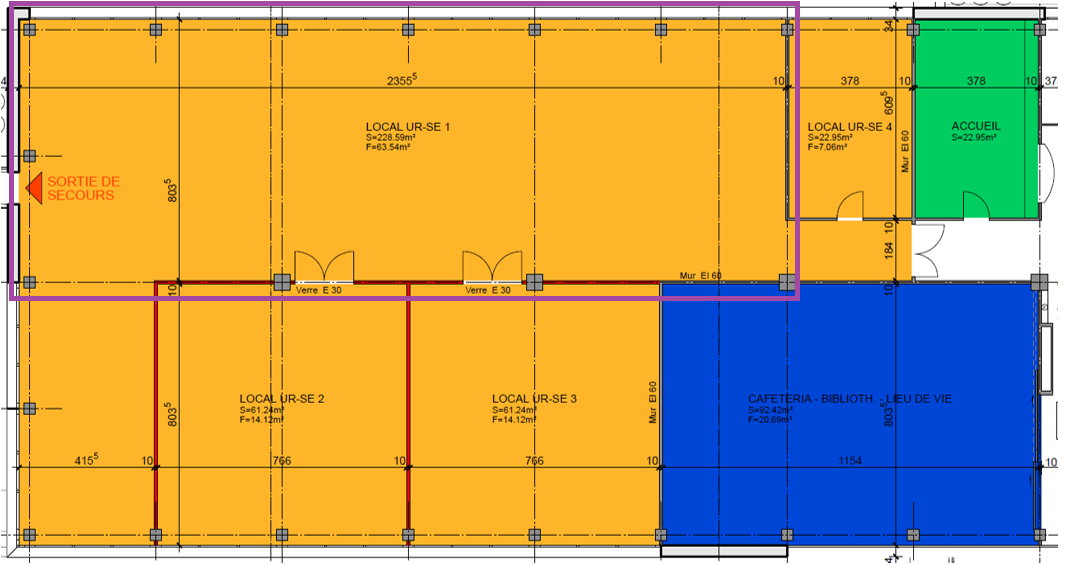
\includegraphics[scale=0.4]{figures/PlanRe.png}
		\caption{Plan réel de la salle}
		\label{fig:PlanRe} %% NOTE: always label *after* caption!
	\end{center}
\end{figure}

La figure \ref{fig:PlanRe} montre le plan modélisé et l'endroit où les mesures seront prises et le placement du maitre et des esclaves.
\begin{figure}[H]
	\begin{center}
		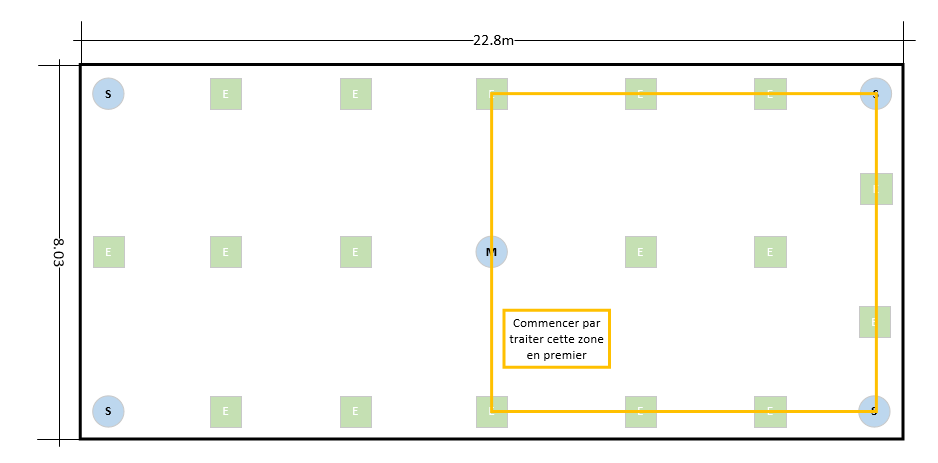
\includegraphics[scale=0.4]{figures/PlanMod.png}
		\caption{Plan indiquant l'endroit des mesures}
		\label{fig:PlanMod} %% NOTE: always label *after* caption!
	\end{center}
\end{figure}

\section{réflexions diverse}
Le choix de l'alforithme n'est pas chose aisée. Même de ssélectionner si on veut faire une régression ou une classification. La regression est quelque chose d'un peu plus compliqué et il est nécessaire d'avoir de très bonnes données ce que je ne sais pas actuellement. Je pense qu'il est préférable dans un premier temps de faire une classification et du coup de donne une zone de positionnement afin de traiter au mieux les datasets. Car le point le plus important c'est la prise de données et depuis la leur traitement. le choix de l'algorithme peut être choisi en fin de processus. 

Il y a possibilité de partir avec SVM pour la classification et ensuite SVR 
Ou alors même KNN pour la classification qui est pas mal cité dans les lectures et qui peut également être utilisé pour la regression.
Et finalement selon certain conseils et recherche concernant ce qui se fait l'algorithme randomforest peut être bien pour débuter car également il permet de faire de la classification ainsi que de la régression.

%\begin{enumerate}
%	\item fgfd
%	\item gdgfd
%\end{enumerate}


%\begin{figure}[H]
%	\begin{center}
%		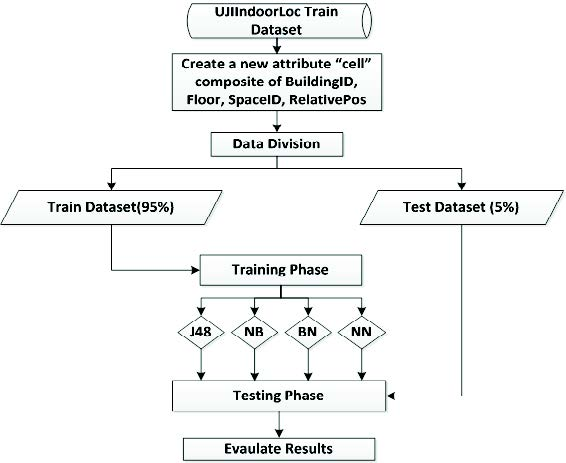
\includegraphics[scale=1]{figures/newattribute.jpg}
%		\caption{The new attribute “cell” construction phase}
%		\label{fig:newAttribute} %% NOTE: always label *after* caption!
%	\end{center}
%\end{figure}

%\todo{Compléter cette partie qui semble importante}

%\chapter{Rapport intérmédiaire : 27.10.2018 au 09.11.2018}

\section{Setup pour la prise de mesure}
Pour effectuer les mesures, il est nécessaire d'effectuer un certain nombre de mesure afin d'avoir un nombre acceptable de données. L'idée est de respecter le plan ci-dessous voir la figure \ref{fig:PlanMod}. Dans un premier temps, les mesures seront effectuée dans une seule moitié du laboratoire. 

Le point rond "M" représente le master, les points ronds "S" représentent les slaves et finalement les points carrés "E" représentent les espions. C'est sur ces derniers que les mesures seront effectuées. 

Il sera nécessaire de prendre 20 mesures sur chaque point. Comme uniquement la première moitié sera considéré les mesures seront faites sur 10 points différents donc 200 données seront à disposition. Une mesure consiste à changer de canal de 1 à 50 et de faire ensuite la moyenne. 

Ces données devront être construites des variables suivantes pour un espion: 
\begin{enumerate}
	\item La coordonnée réelle
	\item Mesures brute pour un canal
	\item Le signal RSSI pour un canal
	\item Erreur pour un canal
	\item le calcul de la coordonnée 
\end{enumerate}

\todo{Afficher ce que reçoit le soft python pour savoir ce qu'il y a exactement car pour le moment c'est un peu flou}

\begin{figure}[H]
	\begin{center}
		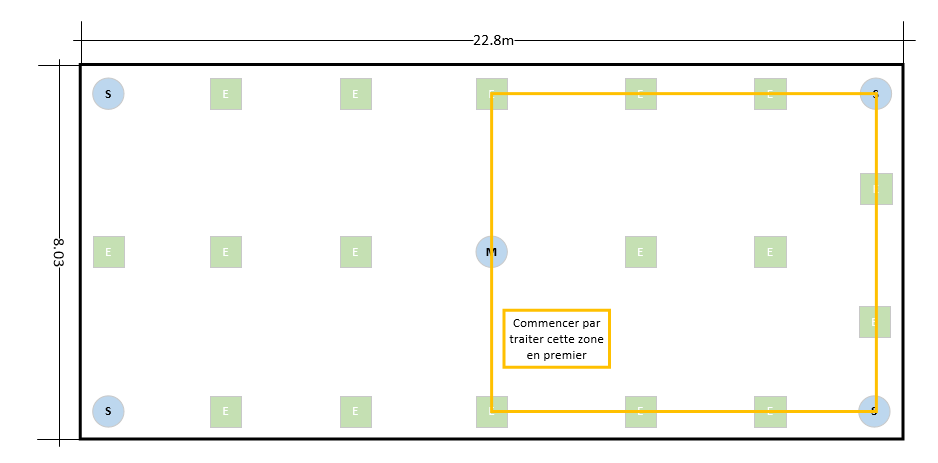
\includegraphics[scale=0.5]{figures/PlanMod.PNG}
		\caption{Montre le setup pour la prise de mesure}
		\label{fig:PlanMod} %% NOTE: always label *after* caption!
	\end{center}
\end{figure}

Le plan de la figure \ref{fig:PlanMod} et un simplification du plan réel de la figure \ref{fig:PlanRe}.

\begin{figure}[H]
	\begin{center}
		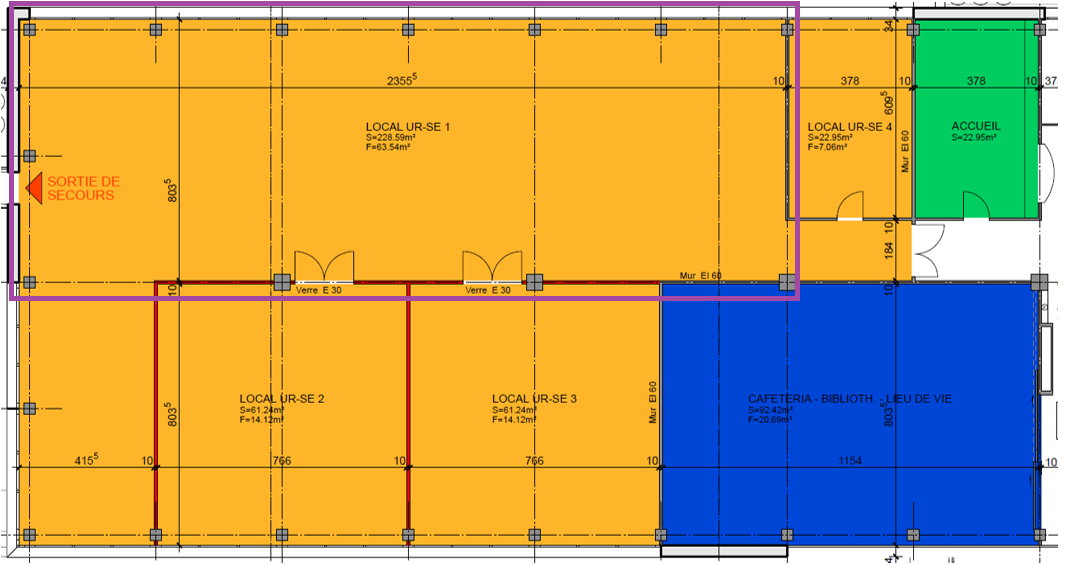
\includegraphics[scale=0.5]{figures/PlanRe.PNG}
		\caption{Montre le plan réel du laboratoire}
		\label{fig:PlanRe} %% NOTE: always label *after* caption!
	\end{center}
\end{figure}

\section{Reprise du soft python de Michael}
Le programme python est relié au Master du réseau LoRa. Il ordonne juste au master de faire un série de mesure. Dès que le master reçois une mesure, il passe le résultat au python qui le stock en RAM et fais passer ça dans des filtres Dans les données reçues, il y a le canal, la valeur brute de mesure, la RSSI, et l'erreur de fréquence estimée. Il est possible d'avoir les mesures brutes en lisant le logs, normalement elles se trouvent dedans (à vérifier).

Les RSSI sont pour l'échange maitre-escalve mais le spy mesure également un RSSI (probablement un rssi moyen).

Le master récupère toutes les mesures du spy et les transmet au PC. Il y a une partie mesure et une partie transmission. C'est ca qui fait que le protocol est un peu compliqué. Le spy stock dans sa RAM les mesures et ressort tout quand le master le demande. Ca c'est le python qui ordonance tout et c'est le fichier de config qui définit comment.

Les coordonnées sont calculées au niveau du soft python et en fonction de ce qui est rentré comme mesure, cela va dans le PositionSolver.

Il est normalement pas nécessaire de s'occuper du soft embarqué par contre il faut maîtriser les adresses.

Comme nous n'avons pas la dernière version du chip il est possible qu'il y ait certain bugs...

Selon le fichier de config, les mesures sont faites sur plusieurs canaux randomisés (ranging slot number = 40). Ca veut dire en gros 40 canaux et le soft python fait cela : 

\begin{enumerate}
	\item Mesurer sur 40 canaux sur un escalve
	\item Récuperer les data sur les spy
	\item mesurer le deuxième exclave
	\item Récupérer les valeurs
	\item etc...
\end{enumerate}

Si plusieurs spy : \\
mesure esclave 1 ->récupérer  spy1,spy2, sp3 / mesure esclave 2 ->récupérer  spy1,spy2, sp3. Les spy sont indépendant des mesures, ils font que écouter les mesures

La structure et datas reçue dans le python sont là :

\begin{lstlisting}
def new burst available(burst_list) :
'''
Callback when new bursts are available
:param burst_list: list_of_bursts
:return: None

=> It will calculate nodes new positions
'''
for burst in burst list:
position solver.update position_solver(burst)
system_gui.update_burst_info(burst)
\end{lstlisting}

C'est le callback qui est reçu dans lr24\_resolver.py. C'est une liste de burst (en python). C'est une liste d'obket "Burst". Et en gros ca stock toutes les mesures pour un couple master-escalve

Dans ces burst il y a les mesures brutes/ le rssi et l'erreur et ca filtre les piques(le bug du chip)
 
\begin{lstlisting}
for burst in burst list:
	valeurs = burst.values
\end{lstlisting}

valeurs[0, canal] = mesure brute pour un canal donné\\
valeurs[1, canal] = rssi pour un canal donné\\
valeurs[2, canal] = erreur pour un canal\\

Pour effectuer les mesures il y a un bouton start/stop.

Il y a deux dimension pour juste un couple maitre escalve. Après c'est N x éenombre. Deux dimensions car canaux x [ raw, rssi, erreur]

%\begin{lstlisting}
% for i=0 to Array.length(t)-1 do
%\end{lstlisting}


%\begin{enumerate}
%	\item fgfd
%	\item gdgfd
%\end{enumerate}


%\begin{figure}[H]
%	\begin{center}
%		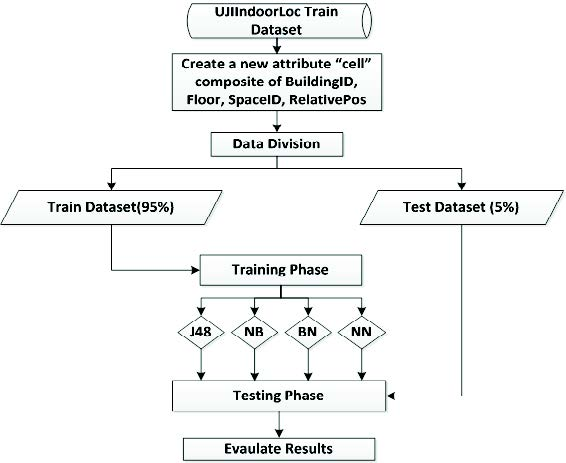
\includegraphics[scale=1]{figures/newattribute.jpg}
%		\caption{The new attribute “cell” construction phase}
%		\label{fig:newAttribute} %% NOTE: always label *after* caption!
%	\end{center}
%\end{figure}

%\todo{Compléter cette partie qui semble importante}


%\chapter{Rapport intermédiaire : 10.11.2018 au 23.11.2018}

\section{Collecte des données}
La collecte des données est un point important de ce travail. Il a été nécessaire de réfléchir quoi prendre et de quel manière. Pour ce faire, Michael Muller qui avait réalisé sa thèse de master concernant le positionnement indoor a réalisé un programme python fonctionnant sur PC et permettant de récupérer les mesures. Ci-dessous sera détaillé un peu plus précisément ce programme afin de pouvoir le prendre en main et réaliser les prises de mesures. 

Ci-dessous, il sera également précisé comment les données ont été structurée afin de pouvoir être utilisée plus tard dans un algorithme d'apprentissage. 

Finalement il sera détaillé comment les mesures ont été effectuées selon le plan du laboratoire.

\subsection{Programme de prise de mesure}
\subsubsection{Architecture}
\subsubsection{Modification du programme original}

\cite{MIC}

\subsection{Structure des données}

\subsection{Plan de mesure}

%\begin{lstlisting}
% for i=0 to Array.length(t)-1 do
%\end{lstlisting}


%\begin{enumerate}
%	\item fgfd
%	\item gdgfd
%\end{enumerate}


%\begin{figure}[H]
%	\begin{center}
%		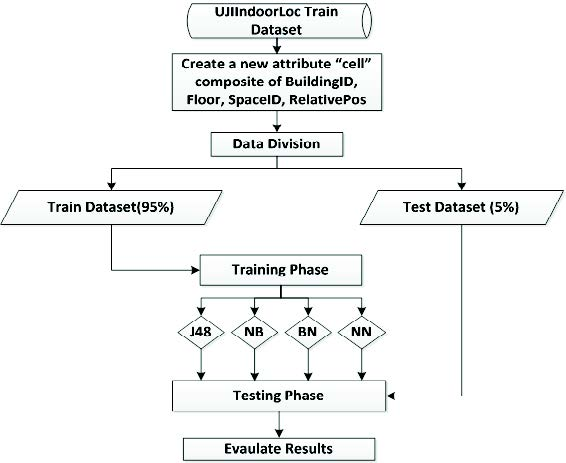
\includegraphics[scale=1]{figures/newattribute.jpg}
%		\caption{The new attribute “cell” construction phase}
%		\label{fig:newAttribute} %% NOTE: always label *after* caption!
%	\end{center}
%\end{figure}

%\todo{Compléter cette partie qui semble importante}


\include{chapter/000_introduction}
\chapter{État de l'art}
Ce chapitre passe en revue les solutions existantes qui parlent d'application des méthodes d'apprentissage pour l'amélioration de la précision de la localisation intérieure. L'exploration de ces sujets va permettre de choisir la solution la plus adaptée pour remplir les objectifs de ce travail.

Pour ce faire, quatre ouvrages ont été étudiés. Les trois premiers traitent du positionnement intérieur aidé avec des algorithmes d'apprentissage (Machine Learning). Le quatrième a été sélectionné, car il traite de la gestion de "outliers", c'est à dire comment détecter des points aberrants et qui pourraient fausser les mesures. 

Grâce à l'étude des structures existantes, une première classification selon le type d'apprentissage et selon les algorithmes de classification utilisés peut être établie. En plus, un aperçu de la façon de détecter les "outliers" est soulevé.

\section{Classification des algorithmes d'apprentissage}
Il existe plusieurs catégories d'estimateur et dans ces catégories, il y a plusieurs algorithmes à choix. La Figure \ref{fig:scikiLearn} permet de sélectionner différents algorithmes en fonction de ce qu'il est nécessaire d'obtenir. On remarque sur cette figure qu'il y a quatre groupes distincts : classification, regression, clustering et dimensionality reduction. En partant depuis le point "start" et en répondant aux différentes questions, cela va proposer un algorithme qui permet de répondre à nos besoins.

\begin{figure}[htp]
 \begin{center}
  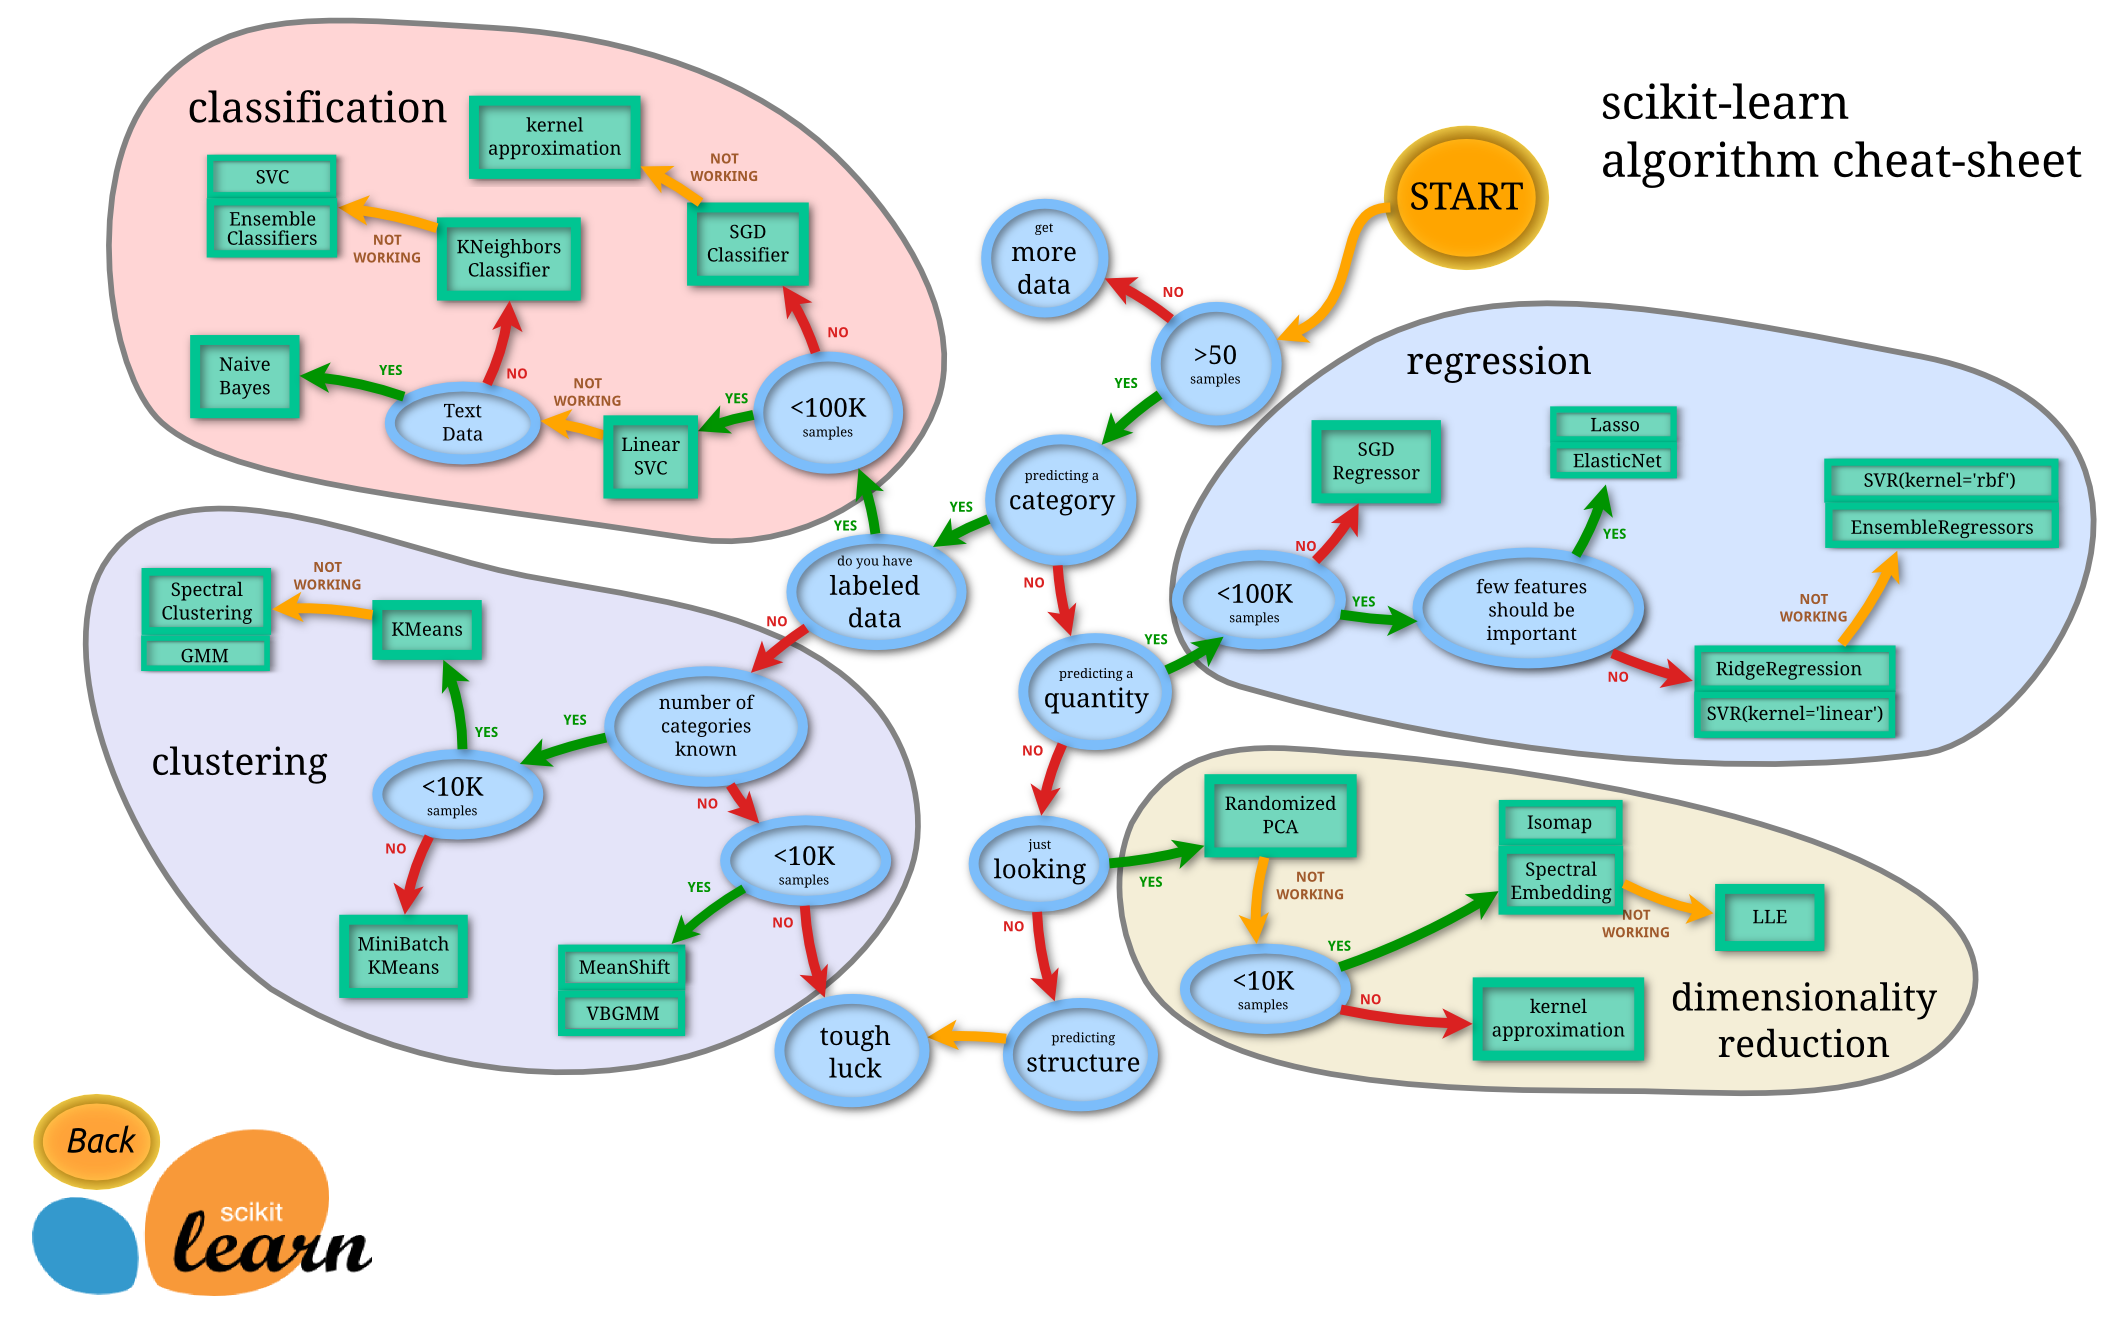
\includegraphics[scale=0.12]{figures/scikiLearn.png}
  \caption{Comment choisir un algorithme ML \cite{scikit}}
  \label{fig:scikiLearn} %% NOTE: always label *after* caption!
 \end{center}
\end{figure}

Dans le cas de ce travail, il y a deux possibilités, soit d'utiliser une classification soit d'utiliser une régression. Dans la Figure \ref{fig:ClassReg}, on peut visualiser la différence entre les deux types d'estimateurs. Dans le cas de la classification, on va apprendre à notre algorithme différentes positions et l'algorithme sera ensuite capable de fournir en sortie une de ses positions. Donc, il sort une région plutôt qu'une coordonnée. Si l'entrainement de l'algorithme a été fait avec un maillage fin alors le résultat sera fin. Lorsqu'un point est détecté, il sera classifié selon la position la plus proche comme on le voit sur la Figure \ref{fig:ClassReg} avec le carré vert et le carré rouge. Dans une régression, la problématique est un peu différente. L'algorithme sera également entrainé avec différentes positions, mais ensuite, par régression l'algorithme va tenter d'estimer la position du nouveau point en calculant sa coordonnée alors que pour une classification il s’agit de positionner ce nouveau point dans une classe. 

\begin{figure}[htp]
 \begin{center}
  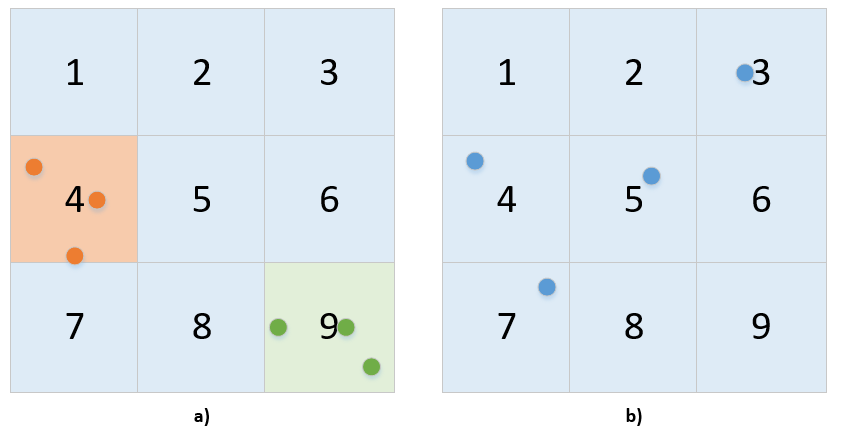
\includegraphics[scale=0.5]{figures/ClassReg.png}
  \caption{a) exemple de classification  b) exemple de régression}
  \label{fig:ClassReg} %% NOTE: always label *after* caption!
 \end{center}
\end{figure}

\section{Algorithme de classification}
Dans cette section, quelques algorithmes de classification utilisés dans ces études \cite{ML_indoor} \cite{CP_RSS} sont brièvement décrits et analysés.

\subsection{Decision Tree}
L'arbre de décisions et une méthode très connue en "machine learning". Il possède des noeuds de décisions (non-terminal), des branches, et des noeuds feuilles (terminal) qui représentent les caractéristiques, condition et les classes. À chaque noeud de décision on sait quelles branches suivre et lorsque l'algorithme atteint un noeud final, le label contenu dans ce même noeud est retourné comme étant la classe. 
L’ID3 de Quinlan et son successeur, C4.5, sont les plus populaires parmi les algorithmes d’arbre de décision \cite{C4_5}.

\subsection{Naïve Bayes}
Le classificateur Naïve Bayes \cite{Bayesian} basé sur le théorème de Bayes est un algorithme d'apprentissage supervisé \cite{DefectPred}. Il est robuste aux données bruyantes, faciles à construire, affiche une grande précision et rapidité lorsqu'il est appliqué à de grandes bases de données et exécute des modèles de classification plus complexes. Par conséquent, il est largement utilisé dans les tâches de classification. Il calcule la probabilité de chaque attribut dans les données en supposant qu'elles sont également importantes et indépendantes les unes des autres. Cette hypothèse est appelée indépendance conditionnelle de classe \cite{KMean_DT} \cite{QUAIL}.

\subsection{Bayesian Network}
L'algorithme de réseau bayésien est largement utilisé pour la classification et est basé sur le théorème de Bayes où la probabilité conditionnelle sur chaque nœud est calculée et forme un réseau bayésien. Il s'appelle également réseau de croyance ou réseau occasionnel. Le réseau bayésien à deux parties nommées qualitatives et quantitatives, qui sont la structure topologique du réseau bayésien et respectivement le tableau de probabilité conditionnelle (CPT) \cite{Bayesian01}.

Le réseau bayésien est un graphe acyclique dirigé où chaque nœud représente un attribut des données et un ensemble de distributions de probabilité. Ces distributions donnent les probabilités pour la valeur de chaque nœud.

\subsection{K-Nearest Neighbor}
Le classificateur K-Nearest Neighbor (K-NN) \cite{ML00} est également connu sous le nom de classificateur basé sur la distance qui classe les instances en fonction de leur similarité. C'est l'un des algorithmes les plus populaires de l'apprentissage automatique. C'est un type d'apprentissage paresseux dans lequel la fonction n'est approchée que localement et tout calcul est retardé jusqu'à la classification. Le point inconnu dans K-NN est assigné à la classe la plus commune parmi ses K-plus proches voisins. Lorsque K = 1, le point inconnu se voit attribuer la classe du point d'apprentissage le plus proche dans l'espace des motifs \cite{ML01}.

\subsection{SMO / SVM}
L'algorithme d'optimisation séquentielle minimale (SMO - Sequential minimal optimization) \cite{ML29} est représenté par John C. Platt pour la formation du classificateur de vecteurs de support à l'aide des noyaux polynomiaux ou RBF. C'est l'un des algorithmes les plus courants pour la classification des grandes marges par SVM. Il remplace globalement toutes les valeurs manquantes et transforme les attributs nominaux en attributs binaires. SVM est une technique de classification basée sur la technologie des réseaux de neuronnes utilisant la théorie de l'apprentissage statistique \cite{ML30}. Il recherche un hyperplan optimal linéaire afin de maximiser la marge de séparation entre la classe positive et la classe négative. En pratique, la plupart des données ne sont pas linéairement séparables; ainsi, pour rendre la séparation possible, la transformation est effectuée à l'aide d'une fonction du noyau. L'entrée est transformée en un espace caractéristique de dimensions supérieures à l'aide d'une cartographie non linéaire. Une décision sur la fonction du Kernel est nécessaire pour implémenter SVM. Le Kernel définit la classe de fonction \cite{ML31}.

\subsection{AdaBoost}
AdaBoost (Adaptive Boosting) \cite{ML32} est un algorithme d'apprentissage d'ensemble. Généralement, il peut être utilisé avec des algorithmes de Machine learning faibles pour améliorer leurs performances. Il est simple à mettre en œuvre, rapide et moins susceptible d'avoir un overfitting. Il améliore les algorithmes de classification instables tels que J48, DecisionStump, etc. L'idée derrière cet algorithme est d'obtenir un classificateur très précis en combinant de nombreux classificateurs faibles. Il fonctionne en exécutant de manière répétée un algorithme d'apprentissage faible donné sur diverses distributions sur les données d'apprentissage, puis en combinant les classificateurs produits par l'apprenant faible en un classificateur composite unique \cite{ML33}. Les classificateurs de l'ensemble sont ajoutés un par un, de sorte que chaque classificateur suivant est entrainé sur des données difficiles pour les membres précédents de l'ensemble. Les poids sont définis sur les instances du jeu de données, en suivant une règle selon laquelle les instances difficiles à classer prennent plus de poids. Cette règle conduit les classificateurs ultérieurs à se concentrer sur eux \cite{ML34}.

\subsection{Bagging}
Le Bagging \cite{ML35} crée des sacs de données de la même taille que le jeu de données d'origine en appliquant une sélection aléatoire à différents sous-ensembles des données d'apprentissage avec de nombreux exemples qui apparaissent plusieurs fois. Ce processus est appelé réplication bootstrap des données d'entrainement. L'idée derrière cette technique est de construire différents classificateurs en utilisant ces sous-ensembles. Chaque sous-ensemble est utilisé pour entrainer un classificateur individuel. Cette approche d'ensemble utilise le nombre de classificateurs a priori \cite{ML35}.

\section{Algorithme de régression}
Dans cette section, quelques algorithmes de régression utilisés dans cette étude \cite{ML_UWB} sont brièvement décrits et analysés.

\subsection{Support Vector Machine pour la régression (SVR)}
Support Vector Machine (SVM) est une méthode d'apprentissage supervisée utilisée pour la classification. Cette méthode peut être étendue pour résoudre des problèmes de régression et cette méthode s'appelle Support Vetor Regression (SVR).

Systeme Vector Regression (SVR) est considéré comme une technique non paramétrique, car il dépend du Kernel. 

Il existe trois implémentations différentes de Support Vector Regression: SVR, NuSVR et LinearSVR. LinearSVR fournit une implémentation plus rapide que SVR, mais ne considère que les noyaux linéaires, tandis que NuSVR implémente une formulation légèrement différente de SVR et de LinearSVR.\cite{scikit}

\subsection{Gaussian Process (GP)}
Gaussian processes a récemment gagné en intérêt du côté des algorithmes d'apprentissage. Cela, car il forme un bon framework pour résoudre des problèmes de régression \cite{ML51}.

C'est une méthode d'apprentissage supervisée pour résoudre des problèmes de régression comme dit ci-dessus, mais également des problèmes de probabilités. 

Les avantages du processus gaussien sont:

\begin{enumerate}
 \item La prédiction interpole les observations (au moins pour les noyaux normaux).
 \item La prédiction est probabiliste (gaussienne) afin que l’on puisse calculer des intervalles de confiance empiriques et décider en fonction de ceux-ci s’il convient de réajuster (adaptation en ligne, adaptation adaptative) la prévision dans une région d’intérêt.
 \item Polyvalent: différents noyaux peuvent être spécifiés. Les noyaux communs sont fournis, mais il est également possible de spécifier des noyaux personnalisés.
\end{enumerate}

Les inconvénients des processus gaussiens sont:

\begin{enumerate}
 \item Ils ne sont pas clairsemés, c’est-à-dire qu’ils utilisent l’ensemble des informations sur les échantillons / caractéristiques pour effectuer la prédiction.
 \item Ils perdent leur efficacité dans les espaces de grandes dimensions, notamment lorsque le nombre de caractéristiques dépasse quelques dizaines.
\end{enumerate} 

\cite{scikit}. 

\section{ Détection d'outliers \cite{ML_indoor}}
Cette section donne un aperçu de la manière de traiter les "outliers - valeurs aberrantes", c'est-à-dire les points qui ne sont pas cohérents lors d'une mesure. Selon Barnet et Lewis \cite{Outliers}, un "outliers" est défini comme étant une observation qui semble incompatible avec le reste d'un ensemble de données.
Garder un "outliers" dans un jeu de données peut amener à de mauvais résultats, il est donc important de les détecter correctement. Il existe différentes méthodes pour déterminer ces "outliers" :

\begin{enumerate}
 \item Grubbs' test : détecte un "outliers" en supposant une distribution normale.
 \item Tietjen-Moore test : C'est une généralisation de Grubbs' test pour détecter de multiple outliers. Il a cependant un inconvénient, il est nécessaire de connaitre le nombre exact d'ouliers.
 \item Generalized Extreme Studentized Deviate (ESD): c'est également une généralisation du test Grubbs', mais il n'est pas nécessaire de connaitre à l'avance le nombre d'ouliers. Ce test nécessite uniquement une limite supérieure pour le nombre suspect d'outliers.\cite{ESD}
\end{enumerate}

\section{Étude des travaux existants}
Les trois documents ne peuvent pas être comparés à proprement dit, car ils traitent de différentes manières. Un parle d'algorithme de classification et compare différents algorithmes existants. Un autre document traite de régression et compare également différents algorithmes. Le dernier document parle de la prédiction conforme (CP - conformal prediction) qui va permettre d'améliorer encore les résultats avec un algorithme choisi.  

C'est pourquoi les documents sont résumés en mettant les points importants en évidence séparément. Ils seront décrits plutôt que comparés. 

\subsection{Analyse comparative de différents algorithmes pour le positionnement intérieur \cite{ML_algo}}
Cette publication parle d'une analyse comparative entre différents algorithmes de "machine learning" pour du positionnement intérieur. L'étude est basée sur un positionnement "fingerprint" ce qui permet de cartographier un endroit à l'aide de la force du signal réceptionné (RSS - Received Signal Strength).
Dans cet article, les algorithmes de "machine learning" sélectionnés sont comparés en termes de précision de positionnement et de temps de calcul. 

Au cours des expériences, la base de données UJIIndoorLoc est utilisée. La classification est effectuée en premier lieu en utilisant le jeu de données d'origine en considérant les valeurs RSS des 520 points d'accès sans fil (WAP - wireless access points) et les nouveaux attributs définis en tant que «cellule» qui composent les attributs : BuildingID, Floor, SpaceID et RelativePos. Ensuite, une nouvelle méthode est proposée: «Séparation déductive pour le positionnement intérieur (DESIP - Deductive Separation for Indoor Positioning)». Dans cette méthode, tout d'abord, seules les informations de bâtiment et les valeurs RSS mesurées à partir de 520 WAP sont utilisées pour la tâche de classification.

Durant les expériences, des algorithmes tels que le plus proche voisin (NN - nearest neighbor), le SMO, l'arbre de décision (J48), Naïve Bayes et Bayes Net sont utilisés. L’algorithme le plus approprié pour la solution du problème de positionnement intérieur est déterminé en comparant la précision et le temps de calcul de chaque approche.

La base de données entière est séparée de telle sorte que 19'937 enregistrements soient réservés à l'apprentissage et 1'111 enregistrements soient réservés aux tests. Il y a 529 caractéristiques qui sont: les coordonnées où sont prises les empreintes digitales WiFi, telles que bâtiment, étage, espace (bureau, laboratoire, etc.), position relative (dans une pièce ou dans un couloir), etc. Le jeu de données d'apprentissage UJIIndoorLoc comprenant les valeurs RSSI de 520 WAP et une autre «cellule» qui comprend les attributs floor, buildingID, spaceID et relative position de l'ensemble de données d'origine est utilisé pour la tâche de classification. Les étapes des expériences utilisant ce jeu de données sont illustrées à la Figure \ref{fig:newAttribute}. Dans un premier temps, le jeu de données (dataset) est séparé en deux groupes. Un groupe est utilisé pour l'apprentissage (train dataset) et l'autre partie est utilisée pour valider le résultat des différents algorithmes (test dataset). Le jeu d'entrainement est utilisé pour quatre différents algorithmes.

\begin{figure}[htp]
 \begin{center}
  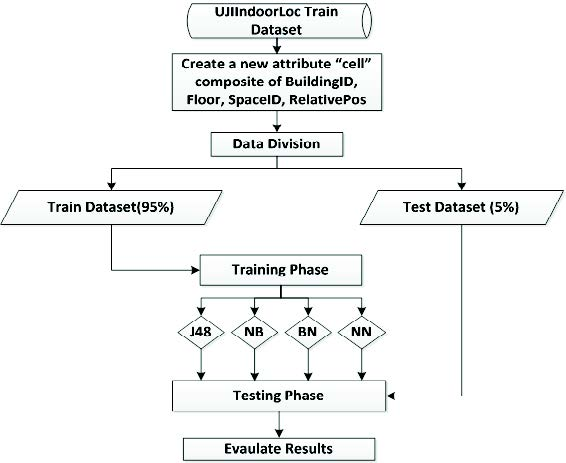
\includegraphics[scale=0.7]{figures/newattribute.jpg}
  \caption{Phase de construction et d'apprentissage \cite{ML_algo}}
  \label{fig:newAttribute} %% NOTE: always label *after* caption!
 \end{center}
\end{figure}

Dans cet article, les algorithmes suivants ont été comparés dans différentes situations: NN, SMO, J48, Naïve Bayes et BayesNet. La classification est effectuée en trois phases (building,floor and region). La première étape est la classification par bâtiment (Figure \ref{fig:builClass}). Le résultat des algorithmes pour cette classification donne BayesNet comme étant le meilleur, car il possède la meilleure précision.

\begin{figure}[htp]
 \begin{center}
  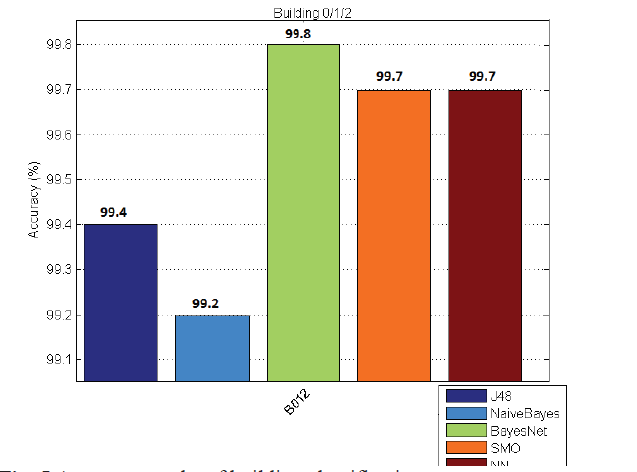
\includegraphics[scale=0.6]{figures/bluildingClassification.png}
  \caption{Résultats des précisons pour la classification par bâtiments \cite{ML_algo}}
  \label{fig:builClass} %% NOTE: always label *after* caption!
 \end{center}
\end{figure}

Suite à cela, la classification a été faite en fonction des étages (floors) (Figure \ref{fig:floorClass}). Dans ce cas, le meilleur algorithme est NN. 

\begin{figure}[htp]
 \begin{center}
  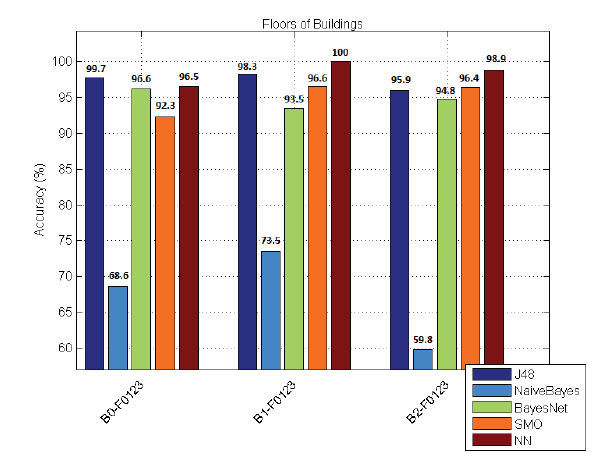
\includegraphics[scale=0.6]{figures/floorClassification.png}
  \caption{Résultats de la précision pour la classification par étage.\cite{ML_algo}}
  \label{fig:floorClass} %% NOTE: always label *after* caption!
 \end{center}
\end{figure}

Et pour la dernière étape (Figure \ref{fig:regionClass}), la classification a été faite en fonction de la région et là encore, c'est l'algorithme NN qui est le meilleur.

\begin{figure}[htp]
 \begin{center}
  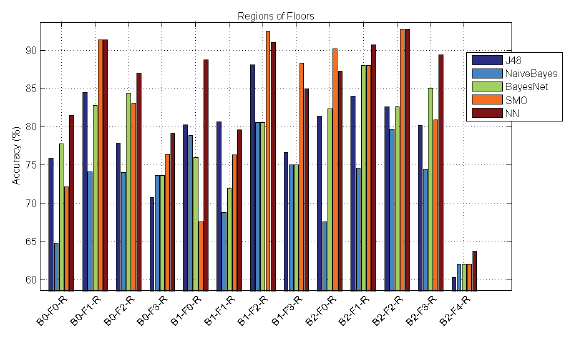
\includegraphics[scale=0.6]{figures/regionClassification.png}
  \caption{Résultats de la précision pour la classification par région. \cite{ML_algo}}
  \label{fig:regionClass} %% NOTE: always label *after* caption!
 \end{center}
\end{figure}

Les deux tableaux (Figure \ref{fig:accuracy} et Figure \ref{fig:time}) permettent d'avoir une vue d'ensemble de tous les algorithmes appliqués et leur performance en termes de précision et de rapidité. L'algorithme NN est le meilleur pour tous les jeux de données au niveau du temps d'exécution. En ce qui concerne la précision, Bayes Net est meilleur pour la classification "building" par contre NN est meilleur dans tous les autres cas.

\begin{figure}[htp]
 \begin{center}
  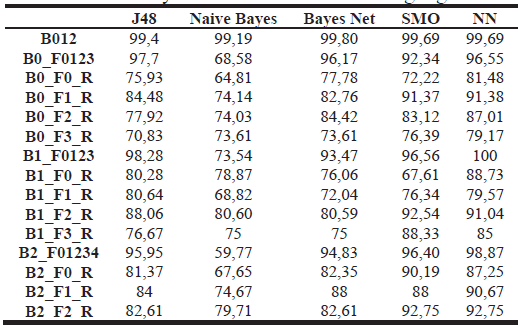
\includegraphics[scale=1]{figures/accuracy.png}
  \caption{Résultat de la précision des algorithmes d'apprentissage.\cite{ML_algo}}
  \label{fig:accuracy} %% NOTE: always label *after* caption!
 \end{center}
\end{figure}

\begin{figure}[htp]
 \begin{center}
  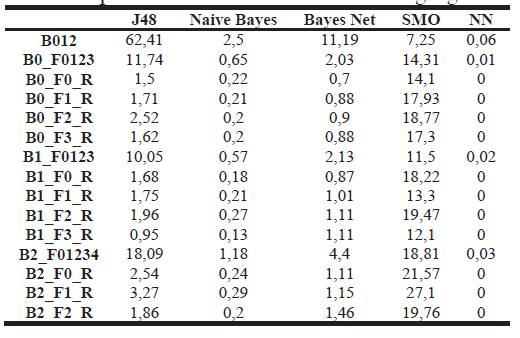
\includegraphics[scale=1]{figures/time.png}
  \caption{Résultats du temps de traitement des algorithmes d'apprentissage\cite{ML_algo}}
  \label{fig:time} %% NOTE: always label *after* caption!
 \end{center}
\end{figure}

Les résultats expérimentaux révèlent que l’algorithme k-Nearest Neighbor (k-NN) est le plus approprié lors du positionnement. En outre, J48 offre des performances quasiment identiques lorsqu'il est utilisé avec des algorithmes itératifs, à savoir AdaBoost et Bagging. Il est à noter que toutes ces méthodes mettent en évidence des classifications. C'est-à-dire que le résultat placera un nouveau point sur l'un des points entrainé et ne donne pas une nouvelle coordonnée comme cela serait le cas d'un résultat par régression. 

\subsection{Machine learning pour diminuer l'erreur de positionnement UWB \cite{ML_UWB}}
Les approches classiques pour faire face au défi de localisation dans des environnements encombrés impliquent généralement d'abord la détection de la condition NLOS (NLOS = pas en ligne de vue), puis la prise de mesures appropriées pour prendre en compte la condition NLOS. Toutefois, la grande variété de matériaux et d’environnements d’exploitation variés peuvent impacter les performances de la mesure de ranging, ce qui indique que la distinction entre LOS et NLOS n’est pas toujours significative. Sur la base de cette observation, ils ont opté pour une approche différente dans cet article. Leur approche utilise des techniques de Machine Learning non paramétriques (SVM et GP) pour estimer l’erreur de "ranging" directement à partir de la forme d’onde reçue, sans aucune connaissance a priori ou a posteriori de la condition NLOS. 

Cette publication traite de la diminution de l'erreur du mode ranging concernant la localisation UWB (Ultra Wide Band). Plusieurs techniques existent pour diminuer l'erreur de positionnement en détectant ce qui est en ligne de vue (LOS) ou non (NLOS). Ici, une autre technique est exploitée et va directement diminuer cette erreur que ça soit en LOS ou en NLOS. Ils appliquent deux classes de régresseurs non paramétriques pour avoir une estimation de l'erreur de mesure. Afin de valider leurs résultats, ils ont fait une vaste campagne de mesures intérieures. Cette technique montre une amélioration de performances significatives dans divers scénarios par rapport aux approches conventionnelles. 

La régression non paramétrique est une forme d'analyse de la régression dans laquelle le prédicteur, ou fonction d'estimation ne prend pas de forme prédéterminée, mais est construite selon les informations provenant des données. La régression non paramétrique exige des tailles d'échantillons plus importantes que celles de la régression basée sur des modèles paramétriques parce que les données doivent fournir la structure du modèle ainsi que les estimations du modèle. \cite{WIKI1}

Ils se sont appuyés sur des outils d'apprentissage (Machine Learning), et proposent deux techniques de régression pour estimer l’erreur de mesure, en se basant uniquement sur la forme d’onde reçue et la distance estimée.

\begin{enumerate}
 \item La première technique utilise une régression SVM (support vector machine) pour trouver un hyperplan qui se rapproche de l'erreur de mesure en fonction des données d'apprentissage. 
 \item La seconde technique utilise un processus gaussien (GP) pour déterminer la distribution a posteriori de l'erreur de mesure, en fonction des données d'apprentissage. 
\end{enumerate}

L'erreur de mesure estimée, associée à une mesure de certitude, peut être transmise à un algorithme de localisation. Leurs techniques de régression présentent l'avantage supplémentaire de pouvoir être appliquées même lorsque les données d'apprentissage ne sont pas étiquetées avec des informations LOS ou NLOS.

Lors des mesures, il existe beaucoup de paramètres qui peuvent créer une erreur. Avec un seul modèle, il est difficile de capturer tous les types de perturbations. Dans cette publication, ils se basent sur 1024 mesures (512 LOS et 512 NLOS) Figure \ref{fig:LosNlos}.

\begin{figure}[htp]
 \begin{center}
  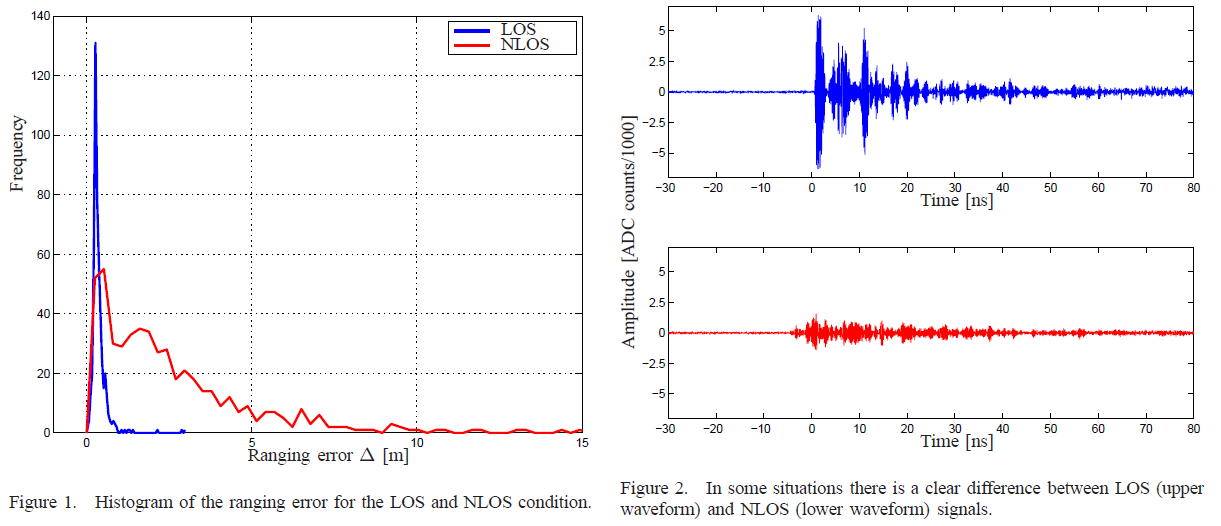
\includegraphics[scale=0.6]{figures/LosNlos.png}
  \caption{Ranging error - LOS and NLOS \cite{ML_UWB}}
  \label{fig:LosNlos} %% NOTE: always label *after* caption!
 \end{center}
\end{figure}

Sur la base d'une vaste campagne de mesures en intérieur avec des radios UWB conformes à la FCC (Federal Communications Commission), ils ont évalué les performances de localisation en termes de probabilité de panne pour différentes stratégies de localisation. Leurs résultats ont révélé que: 

\begin{enumerate}
 \item La minimisation de l1-norme est plus robuste pour faire face aux valeurs aberrantes (outliers) que la minimisation de l2-norme, pour une localisation sans atténuation.
 \item les contraintes peuvent générer des gains significatifs, en particulier lorsque les exigences de localisation ne sont pas trop strictes.
 \item les techniques de régression SVM ou GP offrent des gains de performance supplémentaires pour tous les scénarios considérés.
 \item Les techniques de régression SVM ou GP, combinées à la connaissance des contraintes relatives à l'erreur de "ranging", offrent les meilleures performances pour les scénarios considérés.
\end{enumerate}

\subsection{Amélioration du positionnement en utilisant "conformal prediction" \cite{CP_RSS}}
Pareil que dans les deux précédentes publications, le but est d'améliorer la précision du positionnement intérieur où il n'est pas possible d'utiliser un GPS. Cela toujours en tenant compte des problématiques d'un environnement dynamique avec des personnes qui bougent et de l'environnement complexe avec des murs, etc.. Dans cet article, ils ont validé leur solution dans trois immeubles. Cet article est basé sur un positionnement WIFI fingerprinting et se base sur la force du signal reçu (RSSI).

Pour effectuer les mesures il y a deux phases voir Figure \ref{fig:Fingerprinting}. 

\begin{figure}[htp]
 \begin{center}
  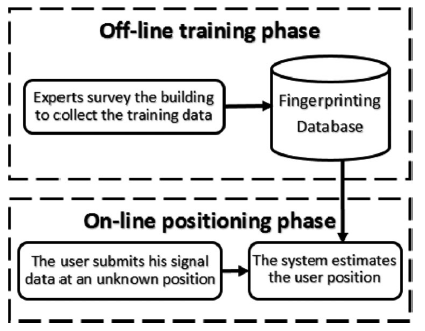
\includegraphics[scale=1]{figures/Fingerprinting.png}
  \caption{Les deux phases du fingerprinting}
  \label{fig:Fingerprinting} %% NOTE: always label *after* caption!
 \end{center}
\end{figure}

La première phase (Off-line training) consiste à décider combien de mesures nous voulons faire (tous les mètres? centimètres?), comment sont prises les mesures (plusieurs mesures sont faites à chaque position) et comment labéliser le signal (souvent labélisé avec la coordonnée réelle). Cette phase est très importante et il est nécessaire de bien réfléchir comment procéder (utiliser un robot par exemple). C'est ce qu'on appelle la phase d'entrainement.

Concernant la seconde phase (on-line positioning), c'est de définir le positionnement. Durant cette phase la partie délicate est de définir quel algorithme utiliser. C'est durant cette phase que les algorithmes seront testés. 

Il existe une compétition comparative pour les positionnements intérieurs (Microsoft IPSN 2014) Figure \ref{fig:Competition}.

Une localisation précise à l'intérieur peut potentiellement transformer la façon dont les gens naviguent à l'intérieur, de la même manière que le GPS a transformé la façon dont les gens naviguent à l'extérieur. Au cours des 15 dernières années, le monde universitaire et l’industrie ont proposé et expérimenté plusieurs technologies de localisation en intérieur, mais nous n’avons pas encore assisté à des déploiements à grande échelle. Ce concours vise à rassembler des technologies de localisation intérieure en temps réel ou quasi réel et à comparer leurs performances dans le même espace. \cite{MICRO}

\begin{figure}[htp]
 \begin{center}
  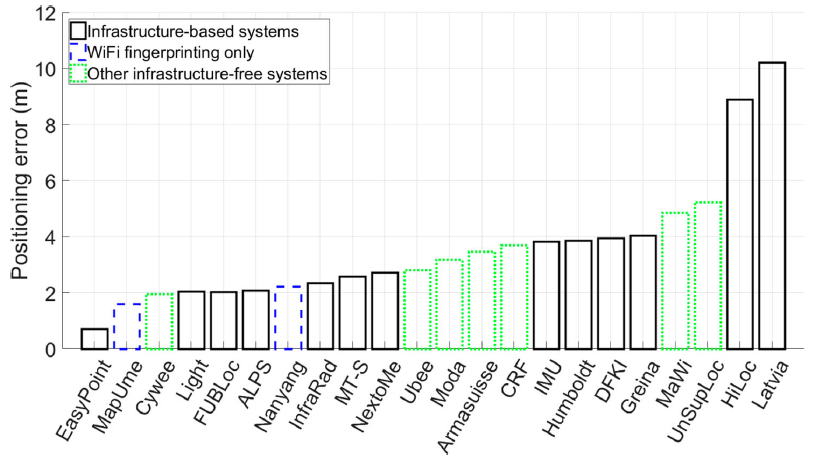
\includegraphics[scale=0.6]{figures/Competition.png}
  \caption{Performance de la précision du fingerprint lors de la compétition Microsoft IPSN 2014 competition \cite{CP_RSS}}
  \label{fig:Competition} %% NOTE: always label *after* caption!
 \end{center}
\end{figure}

Cela permet de mettre en évidence les précisions qui sont obtenues. Les algorithmes qui seront étudiés sont : Weighted K-nearest neighbours (W-KNN), Naïve Bayes Figure \ref{fig:PerfAccu}. Tous les mesures et tests sont basés sur le RSS du WIFI. 

\begin{figure}[htp]
 \begin{center}
  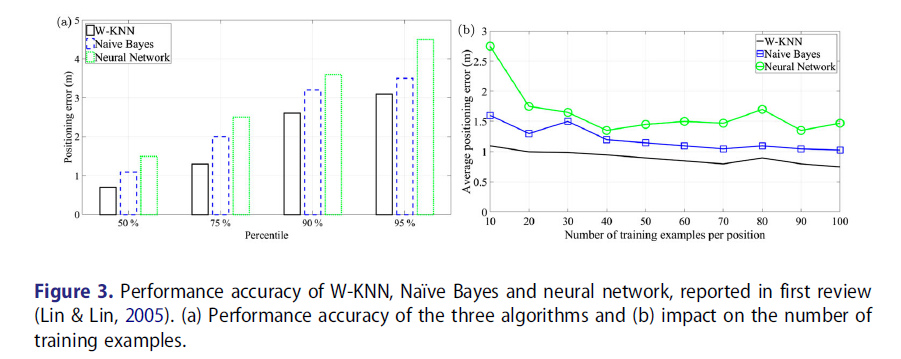
\includegraphics[scale=1]{figures/PerfAccu.png}
  \caption{Performance de la précision de W-KNN, Naïve Bayes et réseau de neurones, mais aussi l'impacte du nombre de données d'entrainement\cite{CP_RSS}}
  \label{fig:PerfAccu} %% NOTE: always label *after* caption!
 \end{center}
\end{figure}

Les mesures ont été effectuées de trois manières différentes (dans un corridor, sur un étage, sur trois étages - voir dans le document  \cite{CP_RSS}). En résumé, la synthèse des trois solutions suggère que, avec uniquement la mesure métrique WiFi RSS, de nombreux algorithmes complexes risquent de ne pas être aussi performants que des algorithmes plus simples. Malgré sa simplicité, W-KNN a excellé dans la plupart des analyses de "fingerprinting". Il convient de noter que le système MapUme, deuxième sur vingt-deux concurrents du concours Microsoft IPSN 2014, utilisait également W-KNN comme principal algorithme. Cependant, l'approche Naïve Bayes améliore sa précision lorsque le nombre d'entrainements est élevé, ce qui indique qu'au-delà du WiFi RSS, des informations supplémentaires seront nécessaires pour améliorer davantage les performances du "fingerprinting".

Une chose qui est également importante c'est la confiance qu'il y a dans un algorithme. Pour cela, cet article a utilisé "conformal prediction (CP)" afin de donner un indice de confiance. Plus la confiance est souhaité, plus il est nécessaire d'avoir de jeu de données. Les avantages d'utiliser l'indice de confiance sont les suivants:

\begin{enumerate}
 \item Chaque prédiction est associée à un indice de confiance et permet de dire combien la prédiction est correcte. 
 \item La prédiction produite par CP est statistiquement correcte sous les paramètres qui ont été choisis dans la phase on-line.
 \item le niveau de confiance peut être ajusté pour produire un ensemble de prédiction plus grand ou plus petit.
\end{enumerate}

Afin de valider leur algorithme, ils ont utilisé trois bancs de test Figure \ref{fig:TestBed}. 

\begin{enumerate}
 \item Royal Holloway : Données récoltées manuellement dans un office standard avec un smartphone
 \item Cambridge : Données récoltées automatiquement par un robot dans un environnement assez idéal.
 \item UJIIndoorLoc : Utilise le dataset public qui couvre une grande surface intérieure basée sur trois bâtiments.
\end{enumerate}

\begin{figure}[htp]
 \begin{center}
  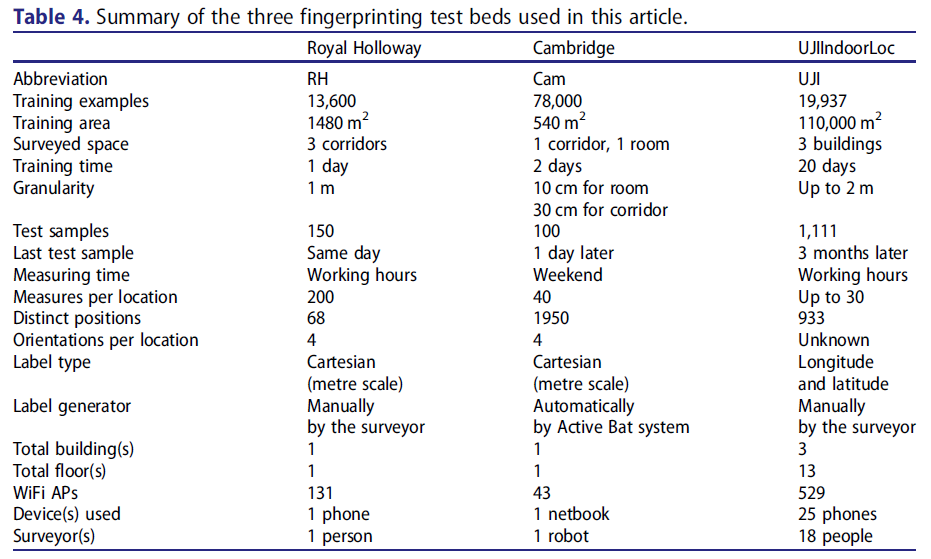
\includegraphics[scale=0.5]{figures/TestBed.png}
  \caption{Summary of the three fingerprinting test beds used in this article \cite{CP_RSS}}
  \label{fig:TestBed} %% NOTE: always label *after* caption!
 \end{center}
\end{figure}

Pour résumer cet article, il propose une nouvelle approche d'apprentissage basé sur la confiance d'un algorithme permettant d'estimer la position de l'utilisateur à l'intérieur avec la force du signal WiFi. Il introduit une mesure de confiance, non seulement utile pour refléter l'incertitude des prédictions de positionnement, mais également capable d'ajuster la taille de l'ensemble de prédictions en conséquence. 

Il a été montré empiriquement que la précision de positionnement était d’environ 2,4 m / probabilité de 75\% avec un banc d’essai normal, environ 70 cm / probabilité de 75\% avec un banc d’essai idéal et d’environ 8,8 m / probabilité de 75\% avec un banc d’essai difficile. 

Ces résultats ont surpassé les algorithmes de Machine Learning sans indice de confiance mis à l'essai sur les mêmes bancs d'essai jusqu'à 20\% plus précis. Si l'on ne tient pas compte de CP, l'algorithme W-KNN est un peu meilleur que Naïve Bayes. 

Les approches présentées dans cet article ne nécessitent pas de carte du bâtiment. Cela pourrait être utile de les avoir afin d'avoir des informations supplémentaires pour supprimer les mauvaises prédictions comme par exemple une personne qui marche dans un mur alors qu'elle est dans le couloir.

\section{Choix et conclusion}
Le choix de l'algorithme suite à l'analyse de l'état de l'art est une tâche difficile. Il est important de garder en tête l'application finale pour laquelle le système sera utilisé, c'est-à-dire, pour faire du positionnement intérieur.

En premier lieu, il est nécessaire de choisir entre un apprentissage par classification ou par régression. Il est clair que pour une utilisation finale un algorithme traitant de la régression comme SVM serait le mieux adapté. Ceci afin d'entrainer le système avec peu de positions et d'estimer les autres positions.

Cependant, il n'est pas vraiment réaliste de démarrer directement avec une technique pareil sans même savoir si les données disponibles sont exploitables. C'est pourquoi la décision a été de démarrer avec un algorithme de classification dans l'optique d'améliorer le système avec un algorithme de régression.

Suite, à l'étude des documents existants, il aurait été possible de sélectionner l'algorithme KNN qui a donnée dans la plupart des cas de bons résultats. Mon choix c'est dirigé vers l'algorithme SVM qui est également bien classé. Ce choix a été fait en grande partie, car il est également cité pour la régression en tant que SVR alors que KNN est uniquement cité pour de la classification. 

%\begin{enumerate}
% \item fgfd
% \item gdgfd
%\end{enumerate}


%\begin{figure}[H]
% \begin{center}
%  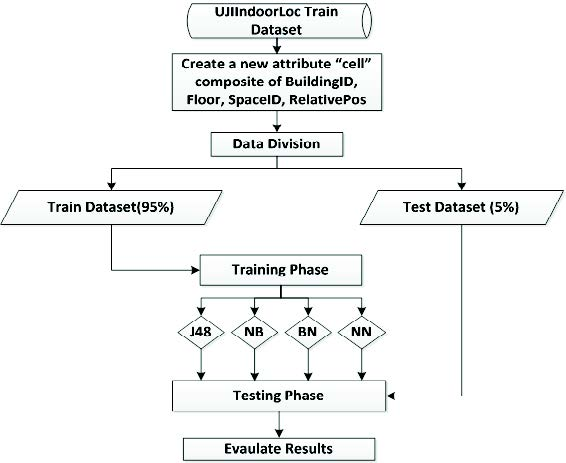
\includegraphics[scale=1]{figures/newattribute.jpg}
%  \caption{The new attribute “cell” construction phase}
%  \label{fig:newAttribute} %% NOTE: always label *after* caption!
% \end{center}
%\end{figure}

%\todo{Compléter cette partie qui semble importante}


\chapter{Prise de mesures}
Ce chapitre traite de la collecte des données qui est un point important de ce travail. Il a été nécessaire de réfléchir à quoi prendre et de quelle manière. Pour ce faire, je me suis servi d'un système de mesures de positionnement intérieur développé par M. Mueller dans le cadre de son travail de Master \cite{MIC}. Ci-dessous, ce programme sera détaillé plus précisément afin de pouvoir le prendre en main et réaliser les prises de mesures. 

Il sera également précisé comment les données ont été structurées afin de pouvoir être utilisée plus tard pour alimenter l'algorithme d'apprentissage. 

Finalement, il sera détaillé comment les mesures ont été effectuées selon le plan du laboratoire.

\section{Plan de mesure}
Un plan de mesure idéal avait été imaginé dans un premier temps pour effectuer les premiers essais, voir sur la Figure \ref{fig:PlanMod}. Ce plan n'a pas pu être réalisé exactement de cette manière dû à la configuration de la salle et de la disposition des établis. Comme décrit ci-dessus, la configuration de la salle pour effectuer les mesures est composée de quatre esclaves (Slaves) placés dans les coins de la pièce à mesurer et le maitre (master) est placé au centre. Ensuite, l'espion est déplacé à différents endroits pour effectuer la prise de mesures voir sur la Figure \ref{fig:mesures}.

\begin{figure}[htp]
 \begin{center}
  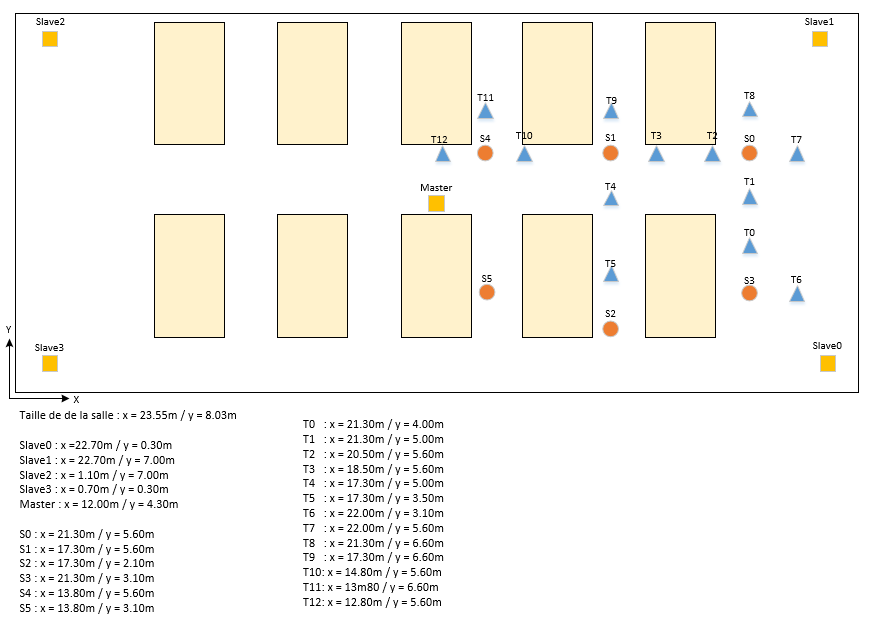
\includegraphics[scale=0.7]{figures/mesures.png}
  \caption{Plan des mesures effectuées et du setup}
  \label{fig:mesures} %% NOTE: always label *after* caption!
 \end{center}
\end{figure}

Afin de mieux comprendre la méthodologie de mesures, un cas réel a été imaginé. C'est-à-dire, que la réflexion a été faite en partant du principe qu'il faut positionner des objets dans un laboratoire et installer le système sans effectuer un quadrillage trop précis afin que le temps d'action soit le plus court possible. 

Les points marqués par Sx (orange foncé) sont les points sur lesquels le système est basé et correspondent à la position de l'espion (spy). Quarante mesures ont été effectuées sur ces six endroits et c'est eux qui seront utilisés pour entrainer le système. Cinq mesures supplémentaires ont été effectuées à ces endroits pour les vérifications. Ces mesures ont été effectuées à des moments différents à l'exception de S5.

Les triangles bleus marqués Tx correspondent à des points de tests et cinq mesures ont été effectuées par point. 

À noter que toutes ces mesures ont été effectuées en positionnant un mat muni d'un carton pour poser la carte de l'espion. Donc à chaque changement de position, il est possible que cette dernière varie de quelques centimètres et que l'orientation de l'antenne soit différente. 

\section{Setup pour la prise de mesures}
Pour effectuer les prises de position, il est nécessaire d'effectuer un certain nombre de mesures afin d'avoir une quantité acceptable de données. Dans un premier temps, l'idée est de se concentrer sur le plan du laboratoire. Pour une première version d'apprentissage, les mesures seront effectuées dans une seule moitié du laboratoire comme indiqué sur la Figure \ref{fig:PlanMod}.

Le point rond "M" représente le maitre, les points ronds "S" représentent les esclaves et finalement les points carrés "E" représentent les espions. C'est sur ces derniers que les mesures seront effectuées. 

Il sera nécessaire de prendre quarante mesures sur chaque point. Comme uniquement la première moitié sera considéré, les mesures seront faites sur six points différents donc 240 données seront à disposition. Une mesure consiste à changer les canaux de 1 à 40.

\begin{figure}[htp]
 \begin{center}
  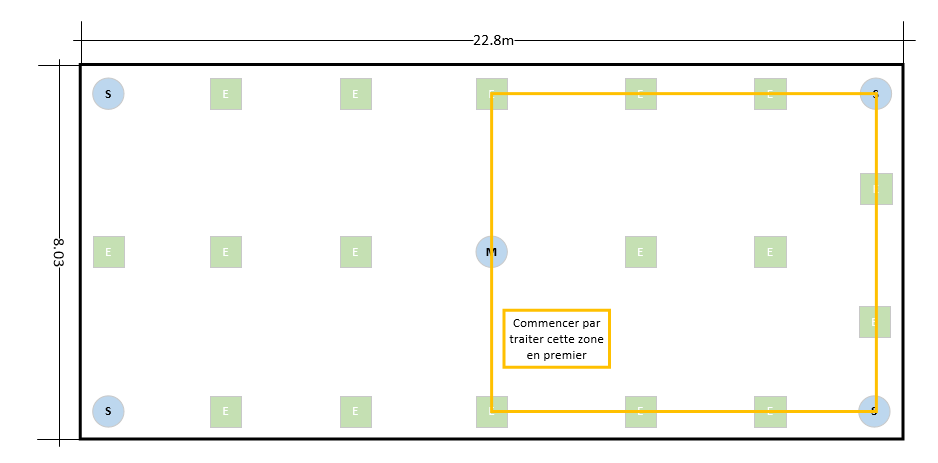
\includegraphics[scale=0.5]{figures/PlanMod.PNG}
  \caption{Montre le setup pour la prise de mesure}
  \label{fig:PlanMod} %% NOTE: always label *after* caption!
 \end{center}
\end{figure}

Le plan de la Figure \ref{fig:PlanMod} et une simplification du plan réel de la Figure \ref{fig:PlanRe}.

\begin{figure}[htp]
 \begin{center}
  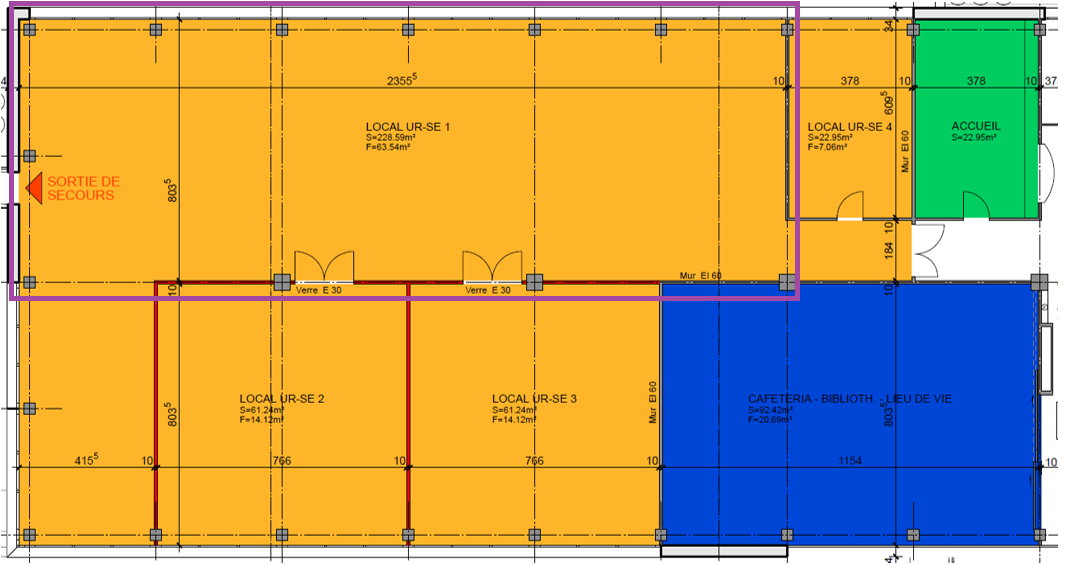
\includegraphics[scale=0.5]{figures/PlanRe.PNG}
  \caption{Montre le plan réel du laboratoire}
  \label{fig:PlanRe} %% NOTE: always label *after* caption!
 \end{center}
\end{figure}

\subsection{Matériel utilisé}
Les cartes utilisées durant ce travail pour les noeuds du système de mesures sont présentées dans la Figure \ref{fig:carte}. Les noeuds sont : les quatre esclaves, le maitre et l'espion. La carte provient de chez Semtech et utilise la radio SX1280, elle est interfacée sur une carte Nucleo-F410RB de chez STMicroelectronics.
 
\begin{figure}[htp]
 \begin{center}
  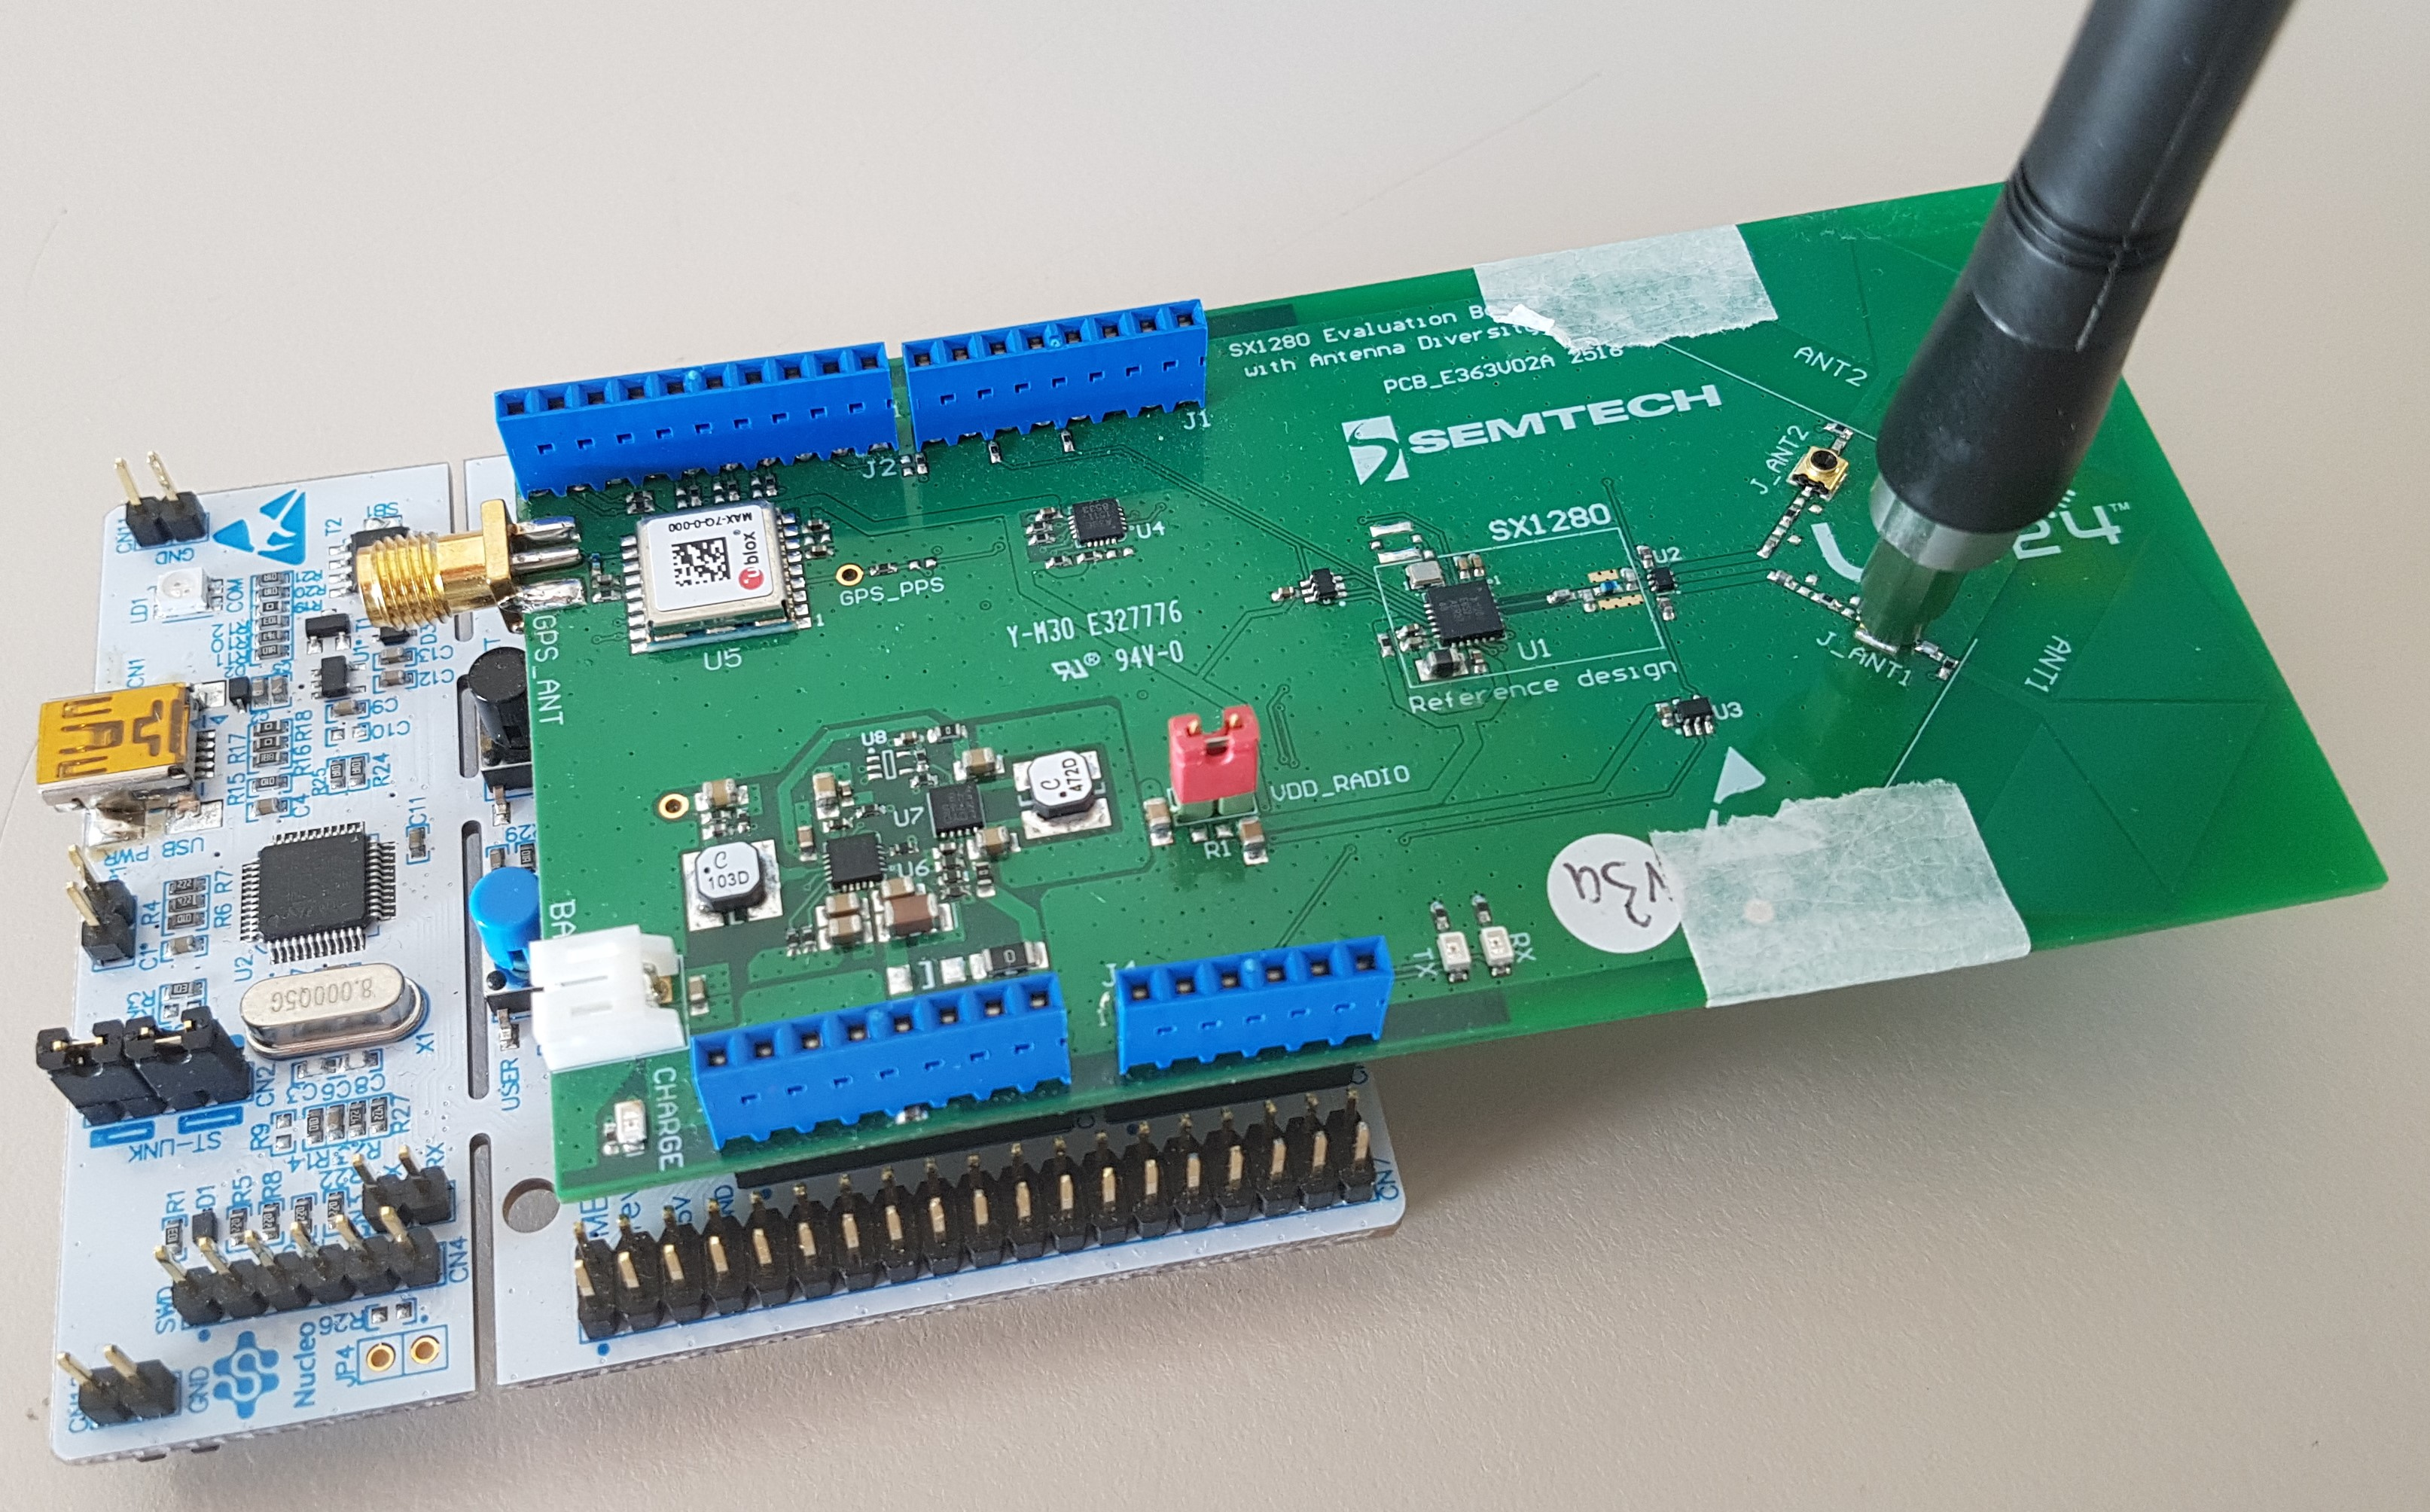
\includegraphics[scale=0.1]{figures/carte.jpg}
  \caption{Montre le plan réel du laboratoire}
  \label{fig:carte} %% NOTE: always label *after* caption!
 \end{center}
\end{figure}

Chaque carte est configurée séparément pour fonctionner selon sa fonction (esclave, maitre ou espion). Il suffit de connecter la carte à un ordinateur et de glisser dans le répertoire qui s'ouvre le fichier "image" correspondant à la fonctionnalité. 

\section{Programme de prise de mesure \cite{MIC}}

Cette section introduit le programme de prise de mesure qui avait été développé. Ce programme permet avant tout d’exploiter pleinement le protocole de localisation, ainsi que les algorithmes de résolution de position. 

Le système peut être composé d’un ou plusieurs esclaves et d’un ou plusieurs maîtres. Les espions font bien entendu partie intégrante également. Le programme effectue des mesures de distance, résout des positions des différents espions et les affiche dans une interface graphique. Le tout est configurable au travers d’un simple fichier de configuration au format texte.

Dans le cadre de ce projet, le fichier de configuration (stage.cfg) contient les informations (position, id,etc.) du "maitre" ainsi que des quatre esclaves. 

Le programme réalisé pour ce démonstrateur a dû être adapté, car il a été conçu pour effectuer des mesures en continu afin d'améliorer au fil du temps le calcul de la position. Cette façon de faire n'est pas utilisable dans le cadre d'un apprentissage à l'aide d'un algorithme.

\subsection{Architecture logicielle}
Pour avoir une meilleure compréhension la structure du programme de prise de mesures, la Figure \ref{fig:archLR24} permet de visualiser les blocs principaux qui interagissent dans le calcul de position.

\begin{figure}[htp]
 \begin{center}
  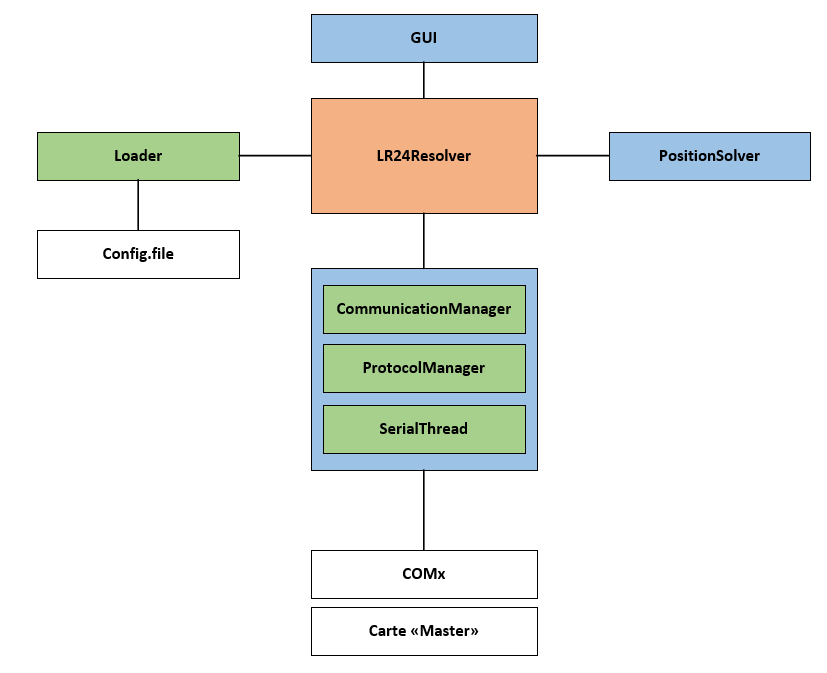
\includegraphics[scale=0.7]{figures/architecture_LR24.PNG}
  \caption{Blocs principaux du logiciel de prise de mesure}
  \label{fig:archLR24} %% NOTE: always label *after* caption!
 \end{center}
\end{figure}

Ci-dessous, une description de chaque bloc est présentée :

\begin{enumerate}
 \item LR24Resolver : Partie centrale du démonstrateur (chef d’orchestre). Il instancie les autres blocs et gère les différents bursts de mesure et de communication).
 \item Loader : Chargé de lire le fichier de configuration et de créer un jeu d’objets utilisables facilement par les autres blocs.
 \item GUI : Interface graphique du système. Il affiche la position des maîtres (carrés verts), des esclaves (cercles verts), des espions (cercles jaunes) et les distances maître-esclave (cercles rouges).
 \item PostionSolver : Chargé de résoudre la position des espions en se basant sur leurs mesures. Il utilise la méthode d’approximation aux moindres carrés avancés.
 \item SerialThread : Communication avec la carte embarquée de type maître. Ce bloc utilise le port série standard. Il lit les données disponibles et les remontes à la couche supérieure. Il transmet aussi les bytes reçus de la couche supérieure vers le port série.
 \item ProtocolManager : Gestion du format du protocole de communication. Cela signifie qu’il transforme les trames reçues en jeu d’objets utilisables, ou alors, il transforme des objets reçus en une trame valide.
 \item CommunicationManager : Gestion des actions (mesure, communication, calibration, etc.). Il reçoit des actions et les exécute au travers du "ProtocolManager".
\end{enumerate}

Une interface graphique est disponible avec le programme lors du lancement. Il est possible de démarrer une mesure, de l'interrompre et de la remettre à zéro, Figure \ref{fig:GUI_LR24}.

\begin{figure}[htp]
 \begin{center}
  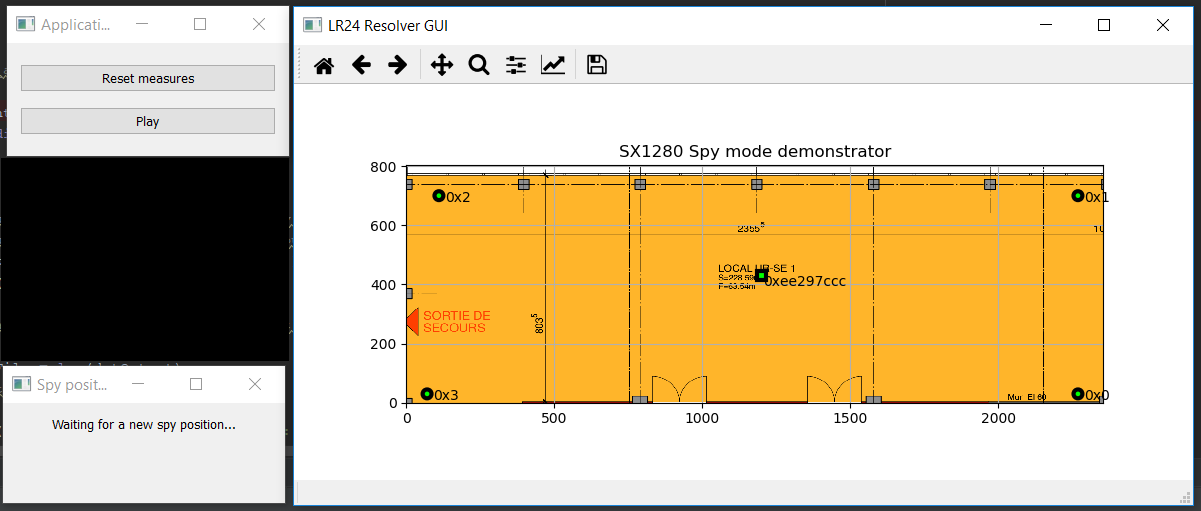
\includegraphics[scale=0.7]{figures/LR24_GUI.png}
  \caption{Interface graphique du soft de prise de mesures}
  \label{fig:GUI_LR24} %% NOTE: always label *after* caption!
 \end{center}
\end{figure}

Ce programme est fait pour ordonner à la carte embarquée "maitre" d'effectuer une série de mesures. Ensuite, dès que le maitre reçoit une mesure de l'espion, il la transfère au programme qui tourne sur le PC. Les mesures réceptionnées sont sous forme de burst. Les informations utiles de ces bursts sont : 

\begin{enumerate}
 \item La provenance du burst de mesure (mesure effectuée sur quel esclave?)
 \item La mesure brute de différence de distance pour chaque esclave et pour quarante canaux de fréquence différents.
 \item La mesure brute du RSSI 
\end{enumerate}

La position de l'espion est calculée au niveau du programme PC (PositionSolver) en fonction des données reçues vu précédemment. Selon le fichier de configuration, les mesures sont faites sur plusieurs canaux (ranging slot number = 40). Le système va effectuer les étapes suivantes en boucle en mesurant séquentiellement chaque esclave: 

\begin{enumerate}
 \item Mesure sur 40 canaux sur un esclave
 \item Récupérer les données sur les maitres
 \item Transmettre les données au niveau du PC
 \item Mesurer le deuxième esclave
 \item Récupérer les données sur le master
 \item Estimation de position quand cela est possible
\end{enumerate}

La fonction qui réceptionne les burst entrant et par conséquent la structure des données se trouve dans le callback ci-dessous :

\begin{lstlisting}
def new burst available(burst_list) :
'''
Callback when new bursts are available
:param burst_list: list_of_bursts
:return: None

=> It will calculate nodes new positions
'''
for burst in burst list:
position solver.update position_solver(burst)
system_gui.update_burst_info(burst)
\end{lstlisting}

Ce callback est reçu dans lr24\_resolver.py. C'est une liste de burst (en python). En résumé, les burst reçus stock toutes les mesures pour un couple maitre-esclave :

valeurs[0, canal] = mesure brute pour un canal donné\.\\
valeurs[1, canal] = rssi pour un canal donné\.\\
valeurs[2, canal] = erreur pour un canal\.\\

Ces données doivent être exploiter pour la suite du travail. 

\subsection{Prise de données brutes}
La prise de données brutes consiste à mémoriser les valeurs brutes des informations de différences de distance fournie par l'espion. Cette mesure provient du fonctionnement des cartes embarquées qui sont configurées pour fonctionner en mode espion. Cette donnée se calcule en faisant Mspy = D1+D2-D3, voir Figure \ref{fig:mesures3}. Lorsque le système possède quatre esclaves, il y aura une mesure par esclave sur chaque fois les quarante canaux. C'est avec ces dernières qu'une position est estimée. 

\begin{figure}[htp]
 \begin{center}
  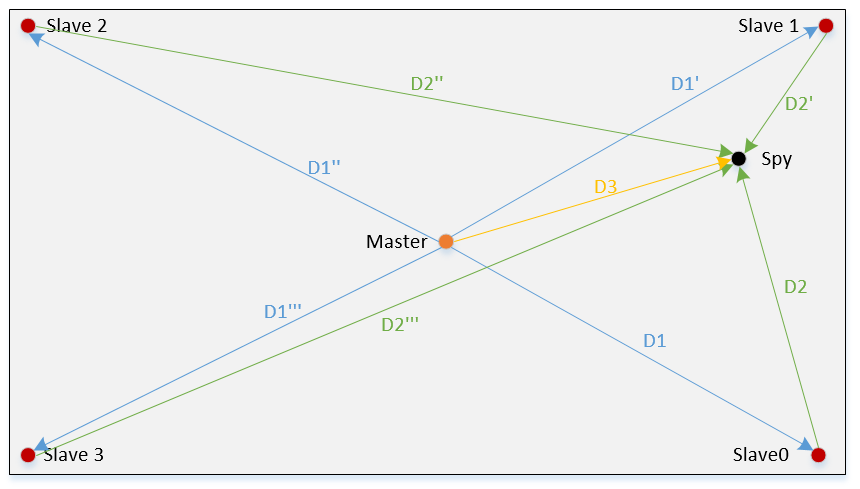
\includegraphics[scale=0.7]{figures/mesures3.png}
  \caption{Fonctionnement du mode spy et signification des mesures brutes}
  \label{fig:mesures3} %% NOTE: always label *after* caption!
 \end{center}
\end{figure}
 
\subsubsection{Modification du programme lr24\_resolver.py}
Le programme Lr24\_resolver.py n'a pas pu être utilisé de la manière dont il avait été créé, car il était destiné à effectuer des mesures continues afin d'améliorer au fil du temps la précision. Dans le cadre de ce projet, il est nécessaire de pouvoir maitriser la prise de mesures ainsi que gérer le nombre d'échantillons enregistrés. La Figure \ref{fig:mesures} montre de quelle manière sont prises les données.

Il a été nécessaire de modifier la fonction new\_burst\_available(burst\_list) du fichier Lr24\_resolver.py afin de mémoriser les huit premiers burst qui arrivent depuis la carte "maitre". De ces "burst" sera uniquement mémorisée la valeur de la différence de distance calculée par l'espion. Cette différence de distance est obtenue grâce au mode "ranging" de la communication LoRa. Un "burst" comprend quarante informations qui sont liées aux quarante canaux de mesures. 

Une fois que les huit bursts ont été reçus, le calcul de position, s’il existe, est mémorisé puis remis à zéro pour la mesure suivante. Il est possible de sélectionner le nombre de mesures désirées grâce à la variable "measures\_count\_des". Quand ce nombre est atteint, le programme s'arrête automatiquement, sinon il continue d'effectuer les mesures.

La fonction "new\_node\_position\_available(node\_pos)" a également été adaptée. Lorsqu'une mesure de position existe, il y a un contrôle qui est effectué afin de s'assurer que les mesures ont été effectuées dans un ordre précis qui est le suivant : Burst reçu de la mesure sur le slave0 (2x) puis du slave1 (2x) puis du slave2 (2x) et finalement du slave3 (2x). Cela afin de ne pas mélanger les données lors de l'apprentissage à l'aide de l'algorithme SVM. 

Finalement, pour que les mesures soient automatiques avec le moins d'interaction possible avec l'utilisateur le fichier gui.py a été modifié pour y ajouter les fonctions software des boutons "stop", "start" et "reset". 

\begin{figure}[htp]
 \begin{center}
  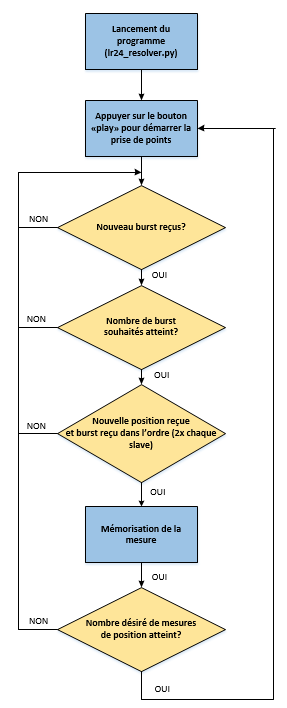
\includegraphics[scale=0.7]{figures/PriseMesures.png}
  \caption{Diagramme expliquant la prise de mesures des valeurs de ranging}
  \label{fig:mesures} %% NOTE: always label *after* caption!
 \end{center}
\end{figure}

\subsubsection{Structure des données}

Dans la Figure \ref{fig:dataStruct} est représenté comment sont structurées les mesures récupérées par le programme python (Lr24\_resolver.py). Il a été nécessaire de faire une réflexion concernant quoi prendre comme mesure et de quelle manière. Il a été décidé de récupérer les informations ci-dessous. A noter qu'un fichier est créé par endroit de mesure, c'est-à-dire qu'a chaque changement de position un nouveau fichier est construit.

\begin{enumerate}
 \item Index : Numéro de la mesure pour un point donné
 \item X1 : Coordonnée X réelle par rapport aux repères de la salle 
 \item Y1 : Coordonnée Y réelle par rapport aux repères de la salle 
 \item X2 : Coordonnée X calculée par le programme python Lr24\_resolver.py après avoir reçus huit bursts
 \item Y2 : Coordonnée Y calculée par le programme python Lr24\_resolver.py après avoir reçus huit bursts
 \item meas : Données brutes de la valeur de "ranging" sur les quarante canaux reçues à chaque burst (8x40 valeurs)
\end{enumerate}

Une décision a été prise à ce niveau de ne pas utiliser le RSSI. Effectivement, la prise de mesures est plus complexe qu'espérée et prend passablement de temps. Le RSSI aurait pu être intégré par la suite en pensant qu'une mesure était rapidement faite, mais ce n'a pas été le cas. 

Sur la Figure \ref{fig:dataStruct} la partie "meas" est séparée en quatre parties, car les bursts sont reçus dans l'ordre deux fois pour l'esclave 0, deux fois pour l'esclave 1, deux fois pour l'esclave 2 et finalement deux fois pour l'esclave 3. 

\begin{figure}[htp]
 \begin{center}
  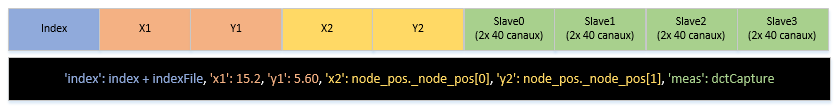
\includegraphics[scale=0.7]{figures/dataStruct.png}
  \caption{Structure des données des mesures de localisation}
  \label{fig:dataStruct} %% NOTE: always label *after* caption!
 \end{center}
\end{figure}

\subsection{Prise de données de positions convergées}
La prise de données des positions convergées est similaire à la prise des mesures brutes sauf que lors du lancement de la mesure, il faut laisser la mesure converger sur sa position finale et la mémoriser sans tenir compte des valeurs brutes des différents canaux.

Cette prise de mesure supplémentaire a été réalisée, car les résultats obtenus uniquement avec les valeurs brutes ne sont pas complétement satisfaisants (voir dans le chapitre suivant). 

\subsubsection{Modification du programme lr24\_resolver.py}
Pareil que ci-dessus, le programme Lr24\_resolver.py n'a pas pu être utilisé comme il avait été créé, car il était destiné à effectuer des mesures continues afin d'améliorer au fil du temps la précision. Dans le cadre de ce projet, il est nécessaire de pouvoir maitriser la prise de mesures. La Figure \ref{fig:mesures2} montre de quelle manière sont prises les données de positions convergées.

Les modifications apportées au logiciel sont similaires à celles détaillées ci-dessus. La seule différence c'est qu'il a été nécessaire de regarder à partir de quel moment la mesure converge et effectuer ce nombre de mesures pour chaque point. La mesure dure environ trois minutes pour obtenir une position convergée ce qui correspond à la réception de 120 burst. 

Le résultat de la position est mémorisé à la suite des 120 burst. 

\begin{figure}[htp]
 \begin{center}
  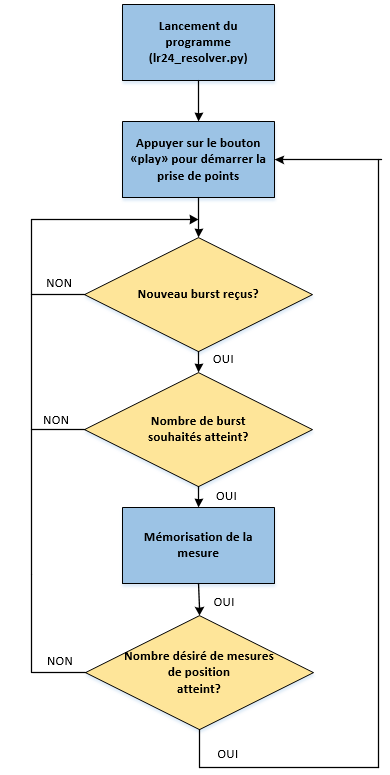
\includegraphics[scale=0.7]{figures/PriseMesures2.png}
  \caption{Diagramme expliquant la prise de mesures des positions convergées}
  \label{fig:mesures2} %% NOTE: always label *after* caption!
 \end{center}
\end{figure}

\subsubsection{Structure des données}
La structure des données voir la Figure \ref{fig:dataStruct2} est similaire à la partie ci-dessus sauf que les données brutes ne sont pas mémorisées, car leur nombre serait trop important. 

\begin{enumerate}
 \item Index : Numéro de la mesure pour un point donné
 \item X1 : Coordonnée X réelle par rapport aux repères de la salle 
 \item Y1 : Coordonnée Y réelle par rapport aux repères de la salle 
 \item X2 : Coordonnée X calculée par le programme python Lr24\_resolver.py après avoir convergée (120 bursts)
 \item Y2 : Coordonnée Y calculée par le programme python Lr24\_resolver.py après avoir convergée (120 bursts)
\end{enumerate}

\begin{figure}[htp]
 \begin{center}
  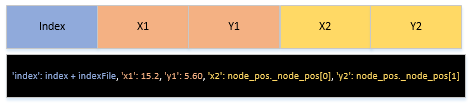
\includegraphics[scale=0.7]{figures/dataStruct2.png}
  \caption{Structure des données de mesures contenant uniquement la valeur des positions convergées}
  \label{fig:dataStruct2} %% NOTE: always label *after* caption!
 \end{center}
\end{figure}



%\begin{lstlisting}
% for i=0 to Array.length(t)-1 do
%\end{lstlisting}


%\begin{enumerate}
% \item fgfd
% \item gdgfd
%\end{enumerate}


%\begin{figure}[H]
% \begin{center}
%  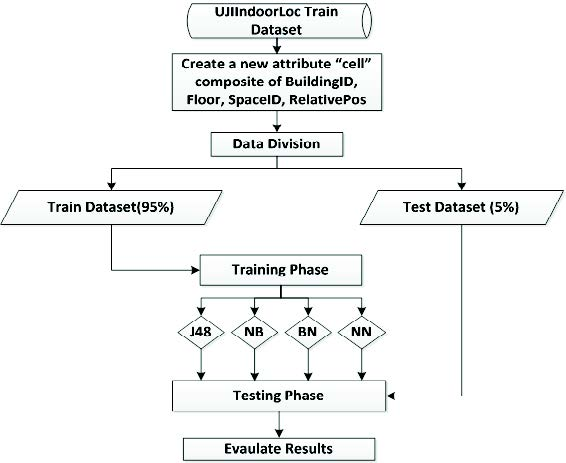
\includegraphics[scale=1]{figures/newattribute.jpg}
%  \caption{The new attribute “cell” construction phase}
%  \label{fig:newAttribute} %% NOTE: always label *after* caption!
% \end{center}
%\end{figure}

%\todo{Compléter cette partie qui semble importante}


\chapter{Traitement des données et classification}
Comme décidé lors de l'analyse de l'état de l'art et les réflexions de départ, la première analyse qui est faite, est de faire de la classification avant de tester les résultats de la régression. 

L'algorithme qui a été sélectionné pour effectuer cette tâche est SVM (Support Vector Machines). Ce chapitre va décrire les différentes étapes qui ont été réalisées pour traiter les données et utiliser l'algorithme.

La programmation a été réalisée sur l'environnement PyCharm PROFESSIONAL 2018.2 et dans le langage Python. Cet environnement m'est le plus familier, car il est étudié dans différents cours, c'est pourquoi mon choix s'est porté sur ce dernier. 

%\begin{figure}[htp]
% \begin{center}
%  
\includegraphics[scale=0.6]{figures/pycharm.png}
%  \caption{Logiciel utilisé pour le développement}
%  \label{fig:pycharm} %% NOTE: always label *after* caption!
% \end{center}
%\end{figure}

\section{Structure du traitement}
Pour le traitement de données pour un apprentissage à l'aide d'un algorithme il est conseillé d'avoir différentes étapes voir Figure \ref{fig:process}. 

\begin{enumerate} 
 \item Acquisition des données : Étape délicate et très importante dans ce projet.
 \item Prétraitement: Étape de traitement sur les données brutes se trouvant dans le jeu de données.
 \item Extraction des caractéristiques : Étape qui consiste à extraire les caractéristiques qui seront utilisées par l’algorithme pour faire la reconnaissance. 
 \item Reconnaissance : Utilisation d’un algorithme pour effectuer la reconnaissance des positions. 
 \item Décision :  Cette étape consiste, si cela est nécessaire, à décider du résultat final à l’aide d’une fusion, cela n'a pas été utilisé.
\end{enumerate}

\begin{figure}[H]
 \begin{center}
  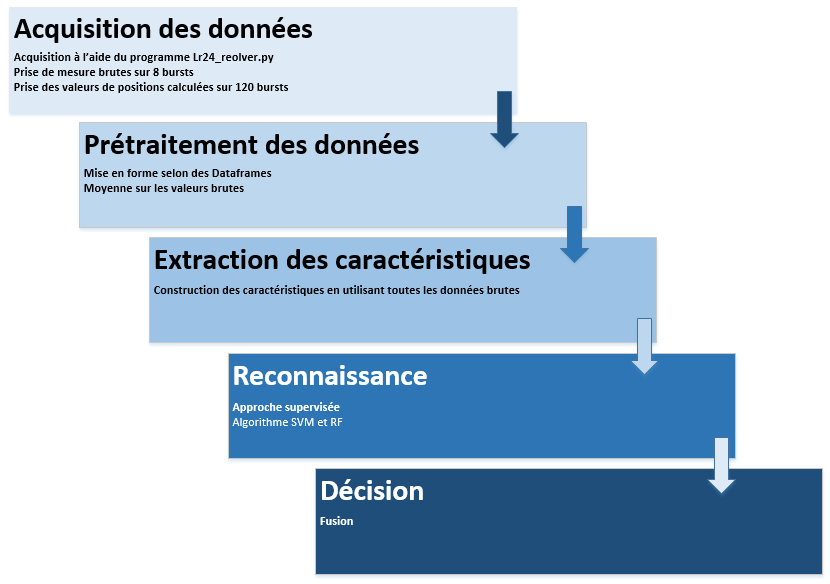
\includegraphics[scale=0.6]{figures/processing.png}
  \caption{Flux de traitement de l'information}
  \label{fig:process} %% NOTE: always label *after* caption!
 \end{center}
\end{figure}

Le premier point est l'acquisition de données qui est décrit au chapitre précédent. C'est une étape primordiale, car c'est grâce à ces données que toute la suite de l'analyse va dépendre. Dans le cadre de ce projet, on remarque vite que si les données ne sont pas prises de manière rigoureuse, cela ne fonctionne pas.

Le prétraitement consiste à utiliser les données disponibles et de les exploiter. Dans un premier temps, les données sont lues depuis un fichier *.npy qui représente des données NumPy. NumPy est une extension du langage de programmation Python, destinée à manipuler des matrices ou tableaux multidimensionnels ainsi que des fonctions mathématiques opérant sur ces tableaux. Plus précisément, cette bibliothèque logicielle libre (open source) fournit de multiples fonctions permettant notamment de créer directement un tableau depuis un fichier ou au contraire de sauvegarder un tableau dans un fichier, et manipuler des vecteurs, matrices et polynômes \cite{WIKI2}. 

Depuis ce fichier, plusieurs traitements sont effectués afin de transformer les données et les mettre dans un format permettant un traitement simple, le format "Dataframe" a été choisi et appartient à la librairie Pandas. Pandas est une bibliothèque écrite pour le langage de programmation Python permettant la manipulation et l'analyse des données. Elle propose en particulier des structures de données et des opérations de manipulation de tableaux numériques et de séries temporelles \cite{WIKI3}. À partir de là, il est possible d'utiliser les données afin d'en extraire des caractéristiques qui est l'étape suivante. Ce point sera détaillé plus loin afin de mieux comprendre ce qui a été utilisé pour que l'algorithme puisse au mieux reconnaitre les différentes positions. 

L'étape de reconnaissance consiste à entrainer un système avec les caractéristiques sélectionnées à partir des données et ensuite de valider que notre algorithme est capable de reconnaitre de nouvelles mesures. Ce point est également détaillé plus bas. 

Finalement, dans ce type d'analyse, il existe souvent une partie décision. Cela peut se faire, car deux algorithmes différents sont utilisés et il est nécessaire de décider quel est le meilleur résultat. Dans le cadre de ce projet, il n'a pas été nécessaire d'utiliser cela, car il n'a pas été possible dans le temps imparti de tester plusieurs techniques et donc la fusion n'était pas utile.

\section{Extraction des caractéristiques}
Ce chapitre traite des caractéristiques qui seront utilisées par l'algorithme afin de déterminer à quelle classe elles appartiennent. La Figue \ref{fig:dataframe} montre comment se présentent les données. Il est possible de les séparer et d'isoler chaque mesure. Chaque mesure est composée des données pour les quarante canaux (colonne : Canal). Les mesures qui peuvent être exploitées pour effectuer la classification sont les mesures brutes de différence de distance (Sx.x). Il serait aussi possible d'exploiter la position fournie par le programme de prise de mesures, mais cette dernière n'est pas assez représentative. C'est pour cette raison que deux types de classification ont été effectués. 

La première consiste à utiliser les données brutes et de travailler avec ces dernières pour extraire d'autres caractéristiques. Les principales qui ont été testées sont décrites ci-dessous.

\begin{enumerate}
 \item Toutes les données (raw) : Cela consiste à prendre toutes les mesures brutes de tous les canaux et de les mettre les unes après les autres. Ce qui veut dire 320 valeurs (quarante canaux fois 2x chaque esclave).
 \item Un canal (raw) : Cette façon de faire est identique à la précédente sauf qu'un seul canal est pris en compte ce qui fait 8 valeurs (un canal fois 2x chaque esclave).
 \item Moyenne : La moyenne est faite sur les quarante canaux par esclave ce qui va donner huit caractéristiques supplémentaires.
 \item Variance : La variance est une mesure qui permet de caractériser la dispersion d'un échantillon. Elle est utilisée pour voir la dispersion des valeurs par esclave sur les quarante canaux. 
 \item Déviation standard : La déviation standard équivaut à la racine carrée de la variance. C'est donc une mesure de dispersion qui est faite également par esclave sur les quarante canaux. 
 \item Quantile : Un quantile correspond à séparer les données en partie de taille égale. C'est-à-dire que chaque partie doit contenir le même nombre de données. Cela est également utilisé pour séparer les données au niveau des canaux pour un esclave.
 \item Médiane : La médiane est en quelque sorte le quantile qui sépare des données en deux parties de même taille. 
 \item covariance : La covariance permet de voir la corrélation entre des variables. Cette mesure est effectuée par esclave sur tous les canaux.  
\end{enumerate}
 
La deuxième consiste à utiliser uniquement la position fournie par le programme de prise de mesure. Cette position est mémorisée après avoir convergée et ce qui fait que les caractéristiques disponibles sont la coordonnée X et la coordonnée Y. Comme il n'y a que deux caractéristiques, il sera difficile d'effectuer différents traitements sur ces données si l'algorithme n'arrive pas différencier les classes. 

Les résultats de ces deux différentes approches seront détaillés au chapitre suivant. 

\begin{figure}[H]
 \begin{center}
  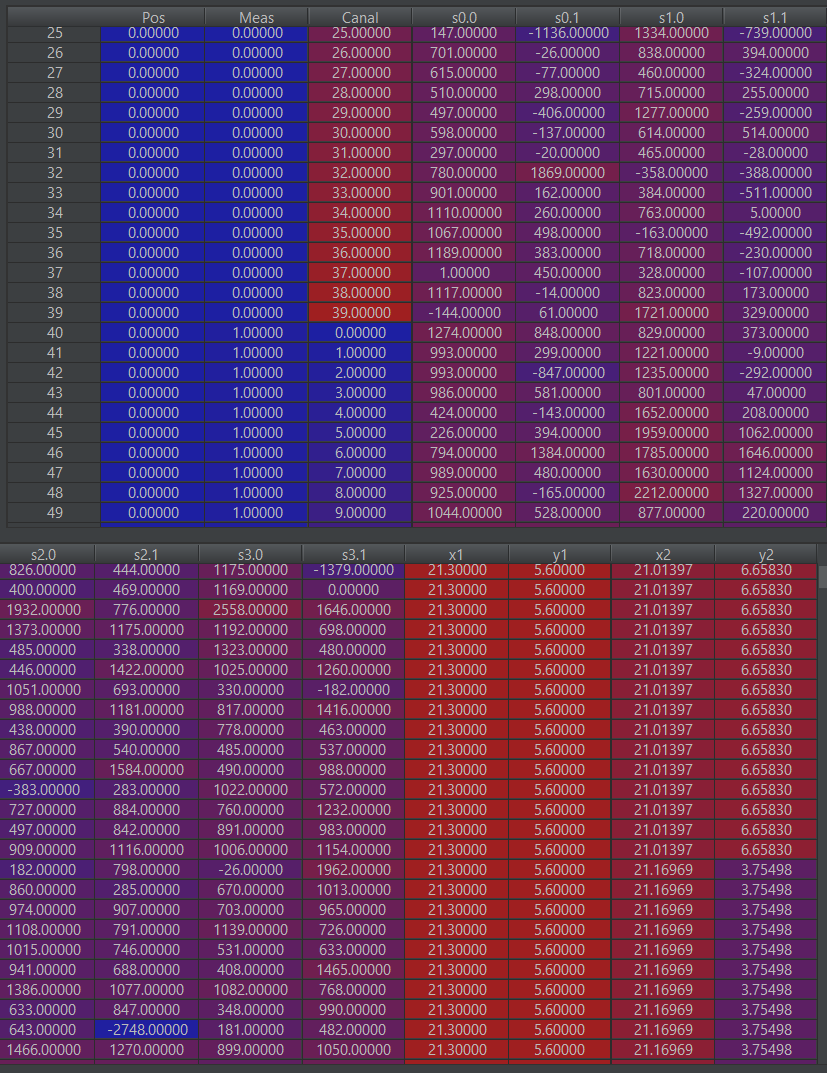
\includegraphics[scale=0.6]{figures/dataframe2.png}
  \caption{Données sous forme de dataframe pour le traitement et l'extraction des caractéristiques}
  \label{fig:dataframe} %% NOTE: always label *after* caption!
 \end{center}
\end{figure}

\section{Reconnaissance - Algorithme}
Le choix de l'algorithme a été fait par rapport à l'état de l'art qui a été effectué en début de projet. Comme déjà mentionné, l'algorithme qui a été retenu est SVM (Support Vector Machine). Cette solution permet de laisser le projet évoluer en utilisant dans un premier temps la solution pour la classification et ensuite en utilisant SVM pour la régression. 

Support Vector Machine est un algorithme supervisé qui permet de faire de la classification en essayant de trouver le meilleur hyperplan. La librairie scikit learn a été utilisée et je me suis servie de sklearn.svm.SVC (System Vector Classification).

L’implémentation de l’algorithme est facile une fois que les labels et les caractéristiques ont été extraits. Dans un premier temps, le canevas de base a été mis en place en utilisant les données brutes des mesures de "ranging". Cela a permis de faire les premiers réglages. 

Afin d'entrainer et de tester l'efficacité de l'algorithme, il est nécessaire de partager les données en trois jeux. Il y a un jeu qui est utilisé pour l'entrainement, un jeu qui est utilisé pour valider l'entrainement qui vient d'être réalisé et un troisième jeu qui sert uniquement pour le résultat final. Dans ce dernier jeu, ce sont des données que l'algorithme n'a jamais vues. La Figure \ref{fig:datasep} permet d'illustrer cette séparation. IL est également possible de voir que les données d'entrainement et de validation vont de pair. Pour ma part, j'ai décidé d'effectuer une cross-validation. C'est-à-dire qu'à chaque lancement le partage des données n'est jamais identique. La seule chose qui est respectée est qu'il y aura toujours 20\% de données pour la validation et 80\% pour l'entrainement. Une autre chose qui est à vérifier c'est que les jeux de données soient balancés. Cela veut dire qu'il doit y avoir le même nombre de données de chaque classe dans chaque jeu. Cela donnerait de mauvais résultats si l'entrainement est fait avec les classes 1,2,et 3 et que la validation se fait avec des données des classes 4 et 5 par exemple. 

\begin{figure}[htp]
 \begin{center}
  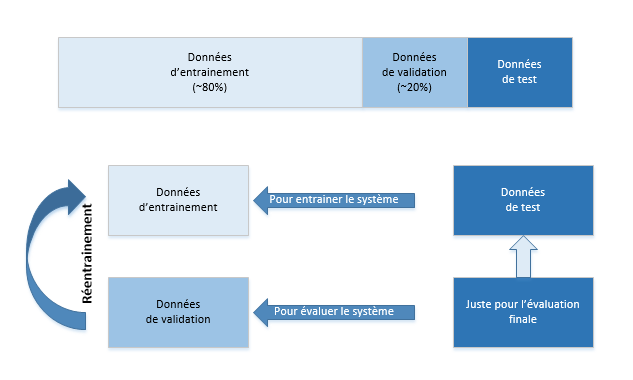
\includegraphics[scale=0.7]{figures/data_separation.png}
  \caption{Partage des données}
  \label{fig:datasep} %% NOTE: always label *after* caption!
 \end{center}
\end{figure}

\subsection{Hyper paramètres}
L'algorithme SVM utilise plusieurs paramètres qu'il a été nécessaire de chercher pour obtenir les meilleurs. Seuls le Kernel, le paramètre C et le paramètre gamma ont été cherchés. Une forte valeur de C tente de minimiser les erreurs de classification des données d'entraînement et une faible valeur essaie de maintenir une classification lisse. Concernant le gamma, plus il est grand , plus la cloche de la gaussienne est étroite voir Figure \ref{fig:c_gamma}. 

\begin{figure}[htp]
 \begin{center}
  \includegraphics[scale=0.7]{figures/c_gamma_param.png}
  \caption{Influence des paramètres C et gamma}
  \label{fig:c_gamma} %% NOTE: always label *after* caption!
 \end{center}
\end{figure}

La première chose qui a été faite a été de trouver le meilleur Kernel pour cette classification. Les Kernel suivants ont été testés : linear, rbf, poly, sigmoid. Celui qui a donné les meilleurs résultats et le Kernel linear.

Suite à cela, un grid-search est effectué sur les paramètres C et gamma. Les meilleurs résultats obtenus sont avec un C égal à 1 et un gamma égal à 0.001. 

\section{Validation et résultats}
Cette section va présenter l'évolution des résultats obtenus au cours du développement. Voici un résumé des données acquises selon la Figure \ref{fig:mesures} : 

\begin{enumerate}
 \item Mesures de "ranging" effectuées sur les points Sx qui correspondent aux points que l'on souhaite retrouver (40x sur chaque point).
 \item Mesures de "ranging" effectuées sur les points Sx à un moment différent que les quarante mesures précédentes (5x sur chaque point).
 \item Mesures de "ranging" effectuées sur les points Tx. Ces points sont pris afin de voir si le plus proche voisin est retrouvé.
 \item Mesures de position effectuées sur les points Sx (40x + 5x sur chaque point).
 \item Mesures de position effectuées sur les points Tx (5x sur chaque point) 
\end{enumerate}

Ces différentes prises de données permettent de faire plusieurs analyses et comprendre de façon plus claire comment le système se comporte.

Les résultats sont évalués à l'aide des matrices de confusion, mais également à l'aide de la mesure de précision, du F1-Score macro et finalement du F1-Score micro. 

La Figure \ref{fig:precisonrecall} montre ce que représente la précision et le rappel. Ces deux notions sont utilisées pour calculer le F1-Score de la manière suivante :

F1\_score = 2((Précision * rappel)/(Précision + rappel))

Le micro ou macro-avarage sont utilisés pour analyser les données de manière différente. Pour le calcul du macro-avarage, il faut additionner les précisions de chaque classe et les diviser par le nombre de classes. Dans ce cas, il se pourrait qu'une classe soit très mauvaise et déséquilibrée, mais que les autres remontent le score. Si maintenant on parle du micro-avarage, le calcul se fait en additionnant les vrais positifs et en les divisant par le nombre total de points. Cette manière de faire va donner un score plus bas si une classe est déséquilibrée \cite{DATASCI}. 

Dans le cadre de cette analyse, toutes les classes possèdent le même nombre de données.

\begin{figure}[htp]
 \begin{center}
  \includegraphics[scale=0.3]{figures/precisionrecall.png}
  \caption{Représentation de la précision et du rappel \cite{WIKI}}
  \label{fig:precisonrecall} %% NOTE: always label *after* caption!
 \end{center}
\end{figure}

\subsection{Résultats en utilisant les données de "ranging"}
Ce chapitre va présenter les résultats qui ont été obtenus à partir des données brutes de "ranging" fournies par le programme de mesures. Plusieurs traitements sont faits sur ces mesures afin d'améliorer les résultats. Le calcul de position est également disponible, mais n'est pas très représentatif, car calculé uniquement à partir de huit valeurs de ranging (deux sur chaque esclave).

Afin d'avoir une meilleure vue de ce que représentent les positions calculées sur peu d'échantillons, la Figure \ref{fig:plotPos} montre le positionnement de ces points calculés par rapport à la position réelle de l'espion. Les gros points de couleurs représentent la position réelle et les petits points de couleurs représentent les positions calculées. La croix noire représente la position du master. On remarque que les petits points sont bien plus espacés que lorsqu’on laisse converger la position (Figrure \ref{fig:plotPosConv}), mais il y a tout de même une séparation entre les ensembles.

\begin{figure}[htp]
 \begin{center}
  \includegraphics[scale=0.8]{figures/plot_pos.PNG}
  \caption{Représentation des points non convergé par rapport aux positions réelles}
  \label{fig:plotPos} %% NOTE: always label *after* caption!
 \end{center}
\end{figure}

La Figure \ref{fig:plotPos} met en évidence un phénomène qui tend à faire rapprocher les points sur la position du maitre. Cet effet qui se trouve dans le laboratoire où les mesures ont été effectuées complique la reconnaissance de position.

Ci-dessous, une énumération des couleurs et de la position associée : 
\begin{enumerate}
 \item Couleur verte (SO) : x = 21.30m / y = 5.60m
 \item Couleur jaune (S1)  : x = 17.30m / y = 5.60m
 \item Couleur bleue (S2) : x = 17.30m / y = 2.10m
 \item Couleur rose (S3) : x = 21.30m / y = 3.10m
 \item Couleur rouge (S4) : x = 13.80m / y = 5.60m 
 \item Couleur noire (S5) : x = 13.80m / y = 3.10m 
\end{enumerate} 

Comme décrit plus haut, toute une série de tests ont été effectués afin de trouver d'une part les meilleurs paramètres et d'autre part de trouver les caractéristiques les plus probantes. Dans tous les essais réalisés, seuls, trois seront détaillés ci-dessous: Résultats obtenus en utilisant uniquement les données de "ranging", résultats obtenus en utilisant uniquement les données de position et finalement présentation de la solution retenue qui utilise la médiane, les données "ranging", les quantiles et la variance.

\subsubsection{Résultat en utilisant toutes les données de ranging brutes}
Le premier test qui a été effectué a été de prendre toutes les données brutes des valeurs de ranging. Cela consiste à prendre chacune des mesures des quatre esclaves sur les quarante canaux et de les mettre les unes à côté des autres pour en créer une caractéristique. Cela est effectué pour chacune des mesures (quarante par position).  

La Figure \ref{fig:matPosSxTRaw} présente le résultat obtenu lorsque l'entrainement est fait avec 32 des 40 mesures sur une même position et testé avec les huit restants. Le résultat obtenu est impressionnant et offre une précision entre 95\% et 100\%. Les positions sont très bien reconnues. La variation de pourcentage pour la reconnaissance vient du fait qu'à chaque lancement, le programme exclut huit autres mesures.

La matrice de confusion représentée est donnée avec des mesures qui ont été faites sur un même point sans bouger l'espion. Le F1-score macro est de 0.9791 et un F1-score micro de 0.9792.  

%Accuracy with optimisation 97.91666666666666 %
%Accuracy 0.9791666666666666
%F1-Score macro : 0.9790849673202615
%F1-Score micro: 0.9791666666666666
\begin{figure}[htp]
 \begin{center}
  \includegraphics[scale=0.5]{figures/mat_pos_Sx_raw.png}
  \caption{Matrice de confusion obtenue en utilisant les points Sx et les caractéristiques de "ranging"}
  \label{fig:matPosSxTRaw} %% NOTE: always label *after* caption!
 \end{center}
\end{figure}

Afin de valider le système, cinq points supplémentaires par position ont été pris durant une autre période et en ayant probablement une position à peine différente. Il faut préciser que les mesures sur la position 5 ont été effectuées au même moment tant pour les quarante que les cinq mesures. C'est pour cette raison que la détection de cette position est très bonne. 

Cela montre une précision de 46.67\% ce qui correspond à 14 positions correctement reconnues sur 30. Ces résultats ne sont pas encourageants, car cela veut dire que sitôt que l'espion est positionné différemment, mais au même endroit cela influence grandement la reconnaissance. Il est donc nécessaire d'effectuer un travaille supplémentaire pour améliorer cette reconnaissance soit niveau prise de mesure soit niveau du travail sur les caractéristiques. Ce qui a été obtenu dans ce test n'était pas ce qui était attendu au vu des résultats obtenus lors de l'entrainement dans la Figure \ref{fig:matPosSxTRaw}.
%toute les raw
%Accuracy with optimisation 46.666666666666664 %
%Accuracy with optimisation 14 sur 30
%Accuracy 0.4666666666666667
\begin{figure}[htp]
 \begin{center}
  \includegraphics[scale=0.5]{figures/mat_pos_SxT_rawall.png}
  \caption{Matrice de confusion obtenue en utilisant les points de tests SxT et les caractéristiques de "ranging" de la 1ère et 2ème mesures de l'esclave}
  \label{fig:matPosSxTRawall} %% NOTE: always label *after* caption!
 \end{center}
\end{figure}

Deux mesures sont effectuées par esclave pour les quarante canaux. L'exemple précédent prend en compte toutes ces mesures. Afin de voir l'effet de ces mesures, un essai a été de prendre uniquement chaque première mesure et ensuite chaque seconde mesure. Étonnement, cela a amélioré les résultats comme le montre la Figure \ref{fig:matPosSxTRaw1}. Les premières mesures offrent de mauvais résultats alors que prendre uniquement les deuxièmes mesures améliore le score. La précision obtenue est de 53.33\% ce qui correspond à 16 positions correctement reconnues sur 30. Difficile à comprendre pourquoi il y a une amélioration. Afin de clarifier cette influence, il serait intéressant de faire plus de deux mesures par escalve et regarder les différents résultats.
%Accuracy with optimisation 53.333333333333336 %
%Accuracy with optimisation 16 sur 30
%Accuracy 0.5333333333333333
\begin{figure}[htp]
 \begin{center}
  \includegraphics[scale=0.5]{figures/mat_pos_SxT_raw1.png}
  \caption{Matrice de confusion obtenue en utilisant les points de tests SxT et les caractéristiques de "ranging" de la 2ème mesure de l'esclave uniquement}
  \label{fig:matPosSxTRaw1} %% NOTE: always label *after* caption!
 \end{center}
\end{figure}

\subsubsection{Résultat en utilisant la position non convergé}
Le résultat qui est présenté ici permet de faire une comparaison entre une mesure qui est convergée (présenté au chapitre suivant) et une mesure qui est calculée uniquement à partir de huit mesures. C'est sans surprise que les résultats qui sont obtenus sont vraiment moins bons.

La Figure \ref{fig:matPosSxTPos} présente le résultat obtenu lorsque l'entrainement est fait avec 32 des 40 mesures sur une même position et testé avec les huit restants. Le résultat obtenu est impressionnant et offre une précision d'environ 70\% contre environ 85\% pour la solution avec les positions convergées. 

La matrice de confusion représentée est donnée avec des mesures qui ont été faites sur un même point sans bouger l'espion. La précision est de 72.91\%, le F1-score macro est de 0.7102 et un F1-score micro de 0.7293.  
%Accuracy with optimisation 72.91666666666666 %
%Accuracy 0.7291666666666666
%F1-Score macro : 0.7102357609710551
%F1-Score micro: 0.7291666666666665
\begin{figure}[htp]
 \begin{center}
  \includegraphics[scale=0.5]{figures/mat_pos_Sx_pos.png}
  \caption{Matrice de confusion obtenue en utilisant les points Sx et la caractéristique de position}
  \label{fig:matPosSxTPos} %% NOTE: always label *after* caption!
 \end{center}
\end{figure}
83.33%

Afin de valider le système, cinq points supplémentaires par position ont été pris durant une autre période et en ayant probablement une position à peine différente. Il faut préciser que les mesures sur la position cinq ont été effectuées au même moment tant pour les quarante que les cinq mesures. C'est pour cette raison que la détection de cette position est très bonne. 

Cela montre une précision de 43.33\% ce qui correspond à 13 positions correctement reconnues sur 30 alors que les résultats pour les positions convergées donnent 83.33\% qui correspond à une reconnaissance correcte de 25 positions sur 30.

%Accuracy with optimisation 43.333333333333336 %
%Accuracy with optimisation 13 sur 30
%Accuracy 0.43333333333333335
\begin{figure}[htp]
 \begin{center}
  \includegraphics[scale=0.5]{figures/mat_pos_SxT_pos.png}
  \caption{Matrice de confusion obtenue en utilisant les points SxT et la caractéristique de position}
  \label{fig:matPosSxTPos} %% NOTE: always label *after* caption!
 \end{center}
\end{figure}

\subsubsection{Meilleur résultat obtenu}
Ce chapitre va présenter le meilleur résultat qui a été obtenu ainsi que les caractéristiques qui ont été utilisées. Pour y arriver, les caractéristiques suivantes ont été testées de manière individuelle :
 
\begin{enumerate}
 \item Toutes les données "ranging" (raw)
 \item Donnée "ranging" d'un canal (raw) 
 \item La moyenne des canaux
 \item La variance sur les canaux
 \item Déviation standard sur les canaux
 \item Quantile effectué sur les canaux
 \item Médiane effectuée sur les canaux 
 \item Covariance des canaux
\end{enumerate}

Ensuite, plusieurs associations ont été faites entre ses différents tests et le meilleur des résultats est obtenu en associant la valeur de la médiane, de la variance, du quantile et des données de "ranging". À noter que pour avoir le meilleur résultat, il a été nécessaire de prendre en compte uniquement la deuxième mesure de ranging sur chaque esclave. Lorsque les différentes caractéristiques sont affichées, il est à noter que l'amplitude des valeurs n'est pas du même ordre et par conséquent pour tenter de les égaliser, la médiane a été multipliée par cinq, le quantile par six et la variance a été divisée par quatre. Cette façon de faire a encore amélioré les résultats pour obtenir ceux présentés ci-dessous.

La Figure \ref{fig:matPosSx} présente le résultat obtenu lorsque l'entrainement est fait avec 32 des 40 mesures sur une même position et testé avec les huit restants. Cela donne de très bonnes précisions qui se situent entre 83\% et 98\%. Les positions sont majoritairement bien reconnues. La variation de pourcentage pour la reconnaissance vient du fait qu'à chaque lancement, le programme exclut huit autres mesures.

La matrice de confusion représentée est donnée avec des mesures qui ont été faites sur un même point sans bouger l'espion. La précision dans ce cas est de 97.92\% avec un F1-score macro de 0.9791 et un F1-score micro de 0.9792. 

\begin{figure}[htp]
 \begin{center}
  \includegraphics[scale=0.5]{figures/mat_pos_Sx.PNG}
  \caption{Matrice de confusion obtenue pour la meilleure solution en utilisant les données des points Sx}
  \label{fig:matPosSx} %% NOTE: always label *after* caption!
 \end{center}
\end{figure}

Maintenant, afin de valider le système cinq points supplémentaires par position ont été pris durant une autre période de la journée et en ayant probablement une position à peine différente. La présentation des précédents résultats montre de très mauvais résultats concernant ce test, mais après le travail effectué et la recherche des meilleures caractéristiques les résultats sont satisfaisants et encourageants. Il faut préciser que les mesures sur la position 5 ont été effectuées au même moment tant pour les quarante que les cinq mesures. C'est pour cette raison que la détection de cette position est excellente. 

Cela montre une précision de 73.33\% ce qui correspond à 22 positions correctement reconnues sur 30. 
%Accuracy with optimisation 73.33333333333333 %
%Accuracy with optimisation 22 sur 30
%Accuracy 0.7333333333333333
\begin{figure}[htp]
 \begin{center}
  \includegraphics[scale=0.5]{figures/mat_pos_SxT.png}
  \caption{Matrice de confusion pour la meilleure solution en utilisant les points de tests SxT}
  \label{fig:matPosSxT} %% NOTE: always label *after* caption!
 \end{center}
\end{figure}

Un dernier test a été réalisé afin de voir si les positions Tx sont bien reconnues par rapport à leur plus proche voisin. La Figure \ref{fig:matPosTx} montre les résultats obtenus lorsque les positions Tx sont utilisées. Les points T1/2/7/8 correspondent à la position S0, T3/4/9 correspondent à la position S1, T5 correspond à la position S2, T0/6 correspondent à la position S3 et finalement, T10/11/12 correspondent à la position S4. Comme attendu, les résultats pour cette classification ne sont pas bons et pas utilisables. La précision obtenue est de 31.25\% ce qui représente une détection correcte de 20 positions sur 64. Pour obtenir ce résultat, on essaie de classifier les positions Tx selon la position entrainée la plus proche. 

\begin{figure}[htp]
 \begin{center}
  \includegraphics[scale=0.5]{figures/mat_pos_Tx.png}
  \caption{Matrice de confusion pour les valeurs de la position convergée avec des points de tests positionnés autour des points entrainés}
  \label{fig:matPosTx} %% NOTE: always label *after* caption!
 \end{center}
\end{figure}

\subsection{Résultats en utilisant les données de position convergées}
Ce chapitre va présenter les résultats qui ont été obtenus à partir des approximations de position fournies par le programme de mesures. Dans cette partie uniquement ces valeurs seront utilisées. Afin d'avoir une meilleure vue de ce que représentent ces positions, la Figure \ref{fig:plotPosConv} montre le positionnement des points calculés par rapport à la position réelle de l'espion. Les gros points de couleurs représentent la position réelle et les petits points de couleurs représentent les positions calculées. La croix noire représente la position du master. 

\begin{figure}[htp]
 \begin{center}
  \includegraphics[scale=0.8]{figures/plot_pos_conv.PNG}
  \caption{Représentation des points convergés par rapport aux positions réelles}
  \label{fig:plotPosConv} %% NOTE: always label *after* caption!
 \end{center}
\end{figure}

La Figure \ref{fig:plotPosConv} met en évidence un phénomène qui tend à faire correspondre les points proches du maitre sur les coordonnées du maitre. Cet effet qui se trouve dans le laboratoire où les mesures ont été effectuées complique la reconnaissance de position. De par cette représentation, il est possible de voir à l'oeil nu la séparation des points. Par contre, il est rapidement possible de se rendre compte que si nous ajoutons des points il sera de plus en plus difficile à différencier les emplacements de base de l'espion.

Ci-dessous, une énumération des couleurs et de la position associée : 
\begin{enumerate}
 \item Couleur verte (SO) : x = 21.30m / y = 5.60m
 \item Couleur jaune (S1)  : x = 17.30m / y = 5.60m
 \item Couleur bleue (S2) : x = 17.30m / y = 2.10m
 \item Couleur rose (S3) : x = 21.30m / y = 3.10m
 \item Couleur rouge (S4) : x = 13.80m / y = 5.60m 
 \item Couleur noire (S5) : x = 13.80m / y = 3.10m 
\end{enumerate} 

La Figure \ref{fig:matPosConvSx} représente le résultat obtenu lorsque l'entrainement est fait avec 32 des 40 mesures sur une même position et testé avec les huit restants. Cela donne de très bonnes précisions qui se situent entre 81\% et 89\%. Comme attendu, les positions proches du maitre (S4 et S5) se confondent et pas conséquent ne sont pas correctement reconnues. Les autres positions sont majoritairement bien reconnues à l'exception de quelques mesures. La variation de pourcentage pour la reconnaissance vient du fait qu'à chaque lancement, le programme exclu huit autres mesures.

\begin{figure}[htp]
 \begin{center}
  \includegraphics[scale=0.5]{figures/mat_pos_conv_Sx_2.PNG}
  \caption{Matrice de confusion pour les valeurs de la position convergée avec des points positionnés à la même place}
  \label{fig:matPosConvSx} %% NOTE: always label *after* caption!
 \end{center}
\end{figure}

Afin de tester l'algorithme fixé, il est entrainé avec les quarante mesures effectuées sur chaque position de l'espion. Ces quarante mesures sont celles utilisées pour définir les meilleurs paramètres et obtenir les meilleurs résultats comme présentés dans la Figure \ref{fig:plotPosConv}. La Figure \ref{fig:matPosConvSxT} présente le résultat final obtenu avec les cinq données de test qui avaient été effectué à la même position que les quarante de l'entrainement. 

La précision obtenue pour ce test est de 83.33\% ce qui correspond à une reconnaissance correcte de 25 positions sur 30. Les positions mal reconnues sont sans surprise les positions S4 et S5.

\begin{figure}[htp]
 \begin{center}
  \includegraphics[scale=0.5]{figures/mat_pos_conv_SxT.png}
  \caption{Matrice de confusion pour les valeurs de la position convergée avec des points de tests positionnés à la même place}
  \label{fig:matPosConvSxT} %% NOTE: always label *after* caption!
 \end{center}
\end{figure}

La Figure \ref{fig:matPosConvTx} montre les résultats obtenus lorsque les positions Tx sont utilisées. Les points T1/2/7/8 correspondent à la position S0, T3/4/9 correspondent à la position S1, T5 correspond à la position S2, T0/6 correspondent à la position S3 et finalement, T10/11/12 correspondent à la position S4. Comme attendu, les résultats pour cette classification ne sont pas bons et pas utilisables. La précision obtenue est de 21.67\% ce qui représente une détection correcte de 13 positions sur 60. Pour obtenir ce résultat on essaie de classifier les positions Tx selon la position entrainée la plus proche. 

\begin{figure}[htp]
 \begin{center}
  \includegraphics[scale=0.5]{figures/mat_pos_conv_Tx.png}
  \caption{Matrice de confusion pour les valeurs de la position convergée avec des points de tests positionnés autour des points entrainés}
  \label{fig:matPosConvTx} %% NOTE: always label *after* caption!
 \end{center}
\end{figure}

\section{Résumé des résultats}
La Figure \ref{fig:result} résume les résultats présentés dans ce rapport. La solution la plus optimiste a été mise en vert. Ce n'est pas celle qui donne les meilleurs résultats au niveau des points SxT, mais malgré cela c'est elle qui offre la plus grande liberté de traitements et d'améliorations. 

La solution qui utilise uniquement la position convergée donne effectivement de bons résultats, mais si le nombre de points est augmenté ils vont commencer de se mélanger et il ne sera plus possible de les différencier. Les positions proches du maitre seront toujours confondues alors qu'avec la solution d'utiliser les données brutes ces positions sont différenciables. Lorsque les données brutes de "ranging" sont utilisées il est possible d'utiliser des traitements sur ces mesures comme la moyenne, la déviation standard, la variance, etc. chose qui n'est pas possible lorsqu'on possède uniquement l'information des coordonnées x et y. 

\begin{figure}[htp]
 \begin{center}
  \includegraphics[scale=0.7]{figures/Resultats.png}
  \caption{Résumé des différents résultats obtenus qui sont présentés dans ce rapport}
  \label{fig:result} %% NOTE: always label *after* caption!
 \end{center}
\end{figure}

Un test supplémentaire a été effectué afin de comparer un autre algorithme. Celui utilisé est "random forest", c'est un des algorithmes cité et utilisé dans l'état de l'art. Les résultats obtenus sont inférieurs avec une précision à 50\% ce qui représente une reconnaissance de 15 positions correctes sur 30 contre 22 sur 30 avec l'algorithme SVM. 

\chapter{Problèmes rencontrés et améliorations}
Ce chapitre traite des problèmes qui ont été rencontrés durant de ce travail d'approfondissement ainsi que des améliorations possibles.

Le projet est basé sur une thèse de Master que Michael Mueller avait réalisé \cite{MIC}. Il avait mis en place un programme permettant de calculer une position dans un local intérieur. Réutiliser ce programme devait permettre d'acquérir facilement des mesures, mais cela n'a pas été le cas. Dans un premier temps, il a été nécessaire de modifier le programme, car le système de prise de mesures n'était pas adapté. Cela dans le sens qu'il effectuait des mesures en permanence en stockant les résultats et en recalculant à chaque fois une position par rapport à toutes les mesures. 

Ce qui a été problématique est la stabilité du système qui à tout moment s'arrête de fonctionner et ne donne plus de résultats utilisables. Les esclaves cessaient de fonctionner de temps en temps et cela faisait qu'une mesure prenait un temps conséquent. Il a aussi été remarqué que lorsque le système fonctionnait durant de longues heures d'affilées les bugs étaient de plus en plus nombreux et le système finissait par n'être plus utilisable. 

De plus, lorsque les mesures de positions convergées ont été réalisée afin d'obtenir une série de mesures sur une position (40 mesures sur les 40 canaux), il fallait une demi-journée. Durant ce temps, il faut sans cesse surveiller le système afin de vérifier que les esclaves ne s'éteignent pas. 

Au niveau des améliorations, il serait important de travailler sur le programme de prise de mesures afin de comprendre pourquoi le système s'arrête parfois. Actuellement, la prise est automatique, mais si un des esclaves s'arrête, il faut le redémarrer et cela ne peut pas être fait de manière automatique. 

Un autre point serait de travailler sur un premier tri des mesures afin d'utiliser uniquement celles qui donnent de bons résultats et supprimer les autres (outlier). Cela permettrait d'avoir de meilleurs résultats finaux. Dans le même ordre d'idée, supprimer les canaux qui seraient bruités.

Concernant la compréhension du système complet, faire les mesures dans un environnement maitrisé où les réflexions/absorption sont limitées (ce qui n'est pas le cas dans le laboratoire) serait d'une grande aide. La quantité de mesures prises doit également être augmentée afin de pouvoir poursuivre le travail et se pencher sur une analyse par régression. 

Une réflexion devrait être faite concernant le positionnement des esclaves et du maitre. Il serait éventuellement intéressant d'ajouter un second maitre et de les placer différemment, par exemple aux extrémités plutôt qu'au centre du local. 

Finalement, l'intégration de la mesure du RSSI pourrait être un candidat très intéressant pour compléter l'analyse et améliorer les prédictions. 

%\begin{lstlisting}
% for i=0 to Array.length(t)-1 do
%\end{lstlisting}


%\begin{enumerate}
% \item fgfd
% \item gdgfd
%\end{enumerate}


%\begin{figure}[H]
% \begin{center}
%  \includegraphics[scale=1]{figures/newattribute.jpg}
%  \caption{The new attribute “cell” construction phase}
%  \label{fig:newAttribute} %% NOTE: always label *after* caption!
% \end{center}
%\end{figure}

%\todo{Compléter cette partie qui semble importante}


%\chapter{Positionnement en utilisant la Regression}

\section{Lecture des données}

\section{Algorithme utilisé}

\section{Structure du traitement}

\section{Choix des caractéristiques utilisées}

\section{Entrainement}

\section{Classification}

\section{Validation de la solution}

\section{Résumé et améliorations à faire}

%\begin{lstlisting}
% for i=0 to Array.length(t)-1 do
%\end{lstlisting}


%\begin{enumerate}
%	\item fgfd
%	\item gdgfd
%\end{enumerate}


%\begin{figure}[H]
%	\begin{center}
%		\includegraphics[scale=1]{figures/newattribute.jpg}
%		\caption{The new attribute “cell” construction phase}
%		\label{fig:newAttribute} %% NOTE: always label *after* caption!
%	\end{center}
%\end{figure}

%\todo{Compléter cette partie qui semble importante}


\chapter{Conclusion}


%\begin{lstlisting}
% for i=0 to Array.length(t)-1 do
%\end{lstlisting}


%\begin{enumerate}
%	\item fgfd
%	\item gdgfd
%\end{enumerate}


%\begin{figure}[H]
%	\begin{center}
%		\includegraphics[scale=1]{figures/newattribute.jpg}
%		\caption{The new attribute “cell” construction phase}
%		\label{fig:newAttribute} %% NOTE: always label *after* caption!
%	\end{center}
%\end{figure}

%\todo{Compléter cette partie qui semble importante}



% following structure:
%	000 => 099 abstract, acknoledgements,...
%	100 => 899 content
%	900 => 999 annexes, ...


%----------------------------------------------------------------------------------------
%	Bibliography
%----------------------------------------------------------------------------------------

%% prints every entry of the bib file -- useful in a state where is no cite
\appendix
\nocite{*}
\printbibliography

%----------------------------------------------------------------------------------------
%	Appendix
%----------------------------------------------------------------------------------------
%% add possible appendix
%\appendix
%\addpart*{Appendix}
%\chapter{Planning}
\begin{figure}[htp]
	\begin{center}
		\includegraphics[width=1\textwidth, angle=90]{../figures/pictures/000-planning.png}
		\caption[Planning]{Planning}
		\label{fig:planning} %% NOTE: always label *after* caption!
	\end{center}
\end{figure}





%----------------------------------------------------------------------------------------
%	\end{document}
%----------------------------------------------------------------------------------------
\end{document}
